%%%%%%%%%%%%%%%%%%don't forget if needed %%%%%%%%%%%%%%%%%%%%%
%\section[toc version]{title version%
%              \sectionmark{head version}}
%\sectionmark{head version}
%%%%%%%%%%%%%%%%%%%%%%%%%%%%%%%%%%%%%%%%%%%%%%%%%%%%%%%%%%%%%%
\def\titcourt{Finite element method}
\def\titlong{Finite element method for the Navier-Stokes-Boussinesq equations using Newton algorithm}
%%%%%%%%%%%%%%%%%%%%%%%%%%%%%%%%%%%%%%%%%%%%%%%%%%%%%%%%%%%%%%%%
\chapter[\titlong]{\titlong%
              \chaptermark{\titcourt}}
\chaptermark{\titcourt}
\label{chap-FEM}
%%%%%%%%%%%%%%%%%%%%%%%%%%%%%%%%%%%%%%%%%%%%%%%%%%%%%%%%%%%%%%%%
%%%%%%%%%%%%%%%%%%%%%%%%%%%%%%%%%%%%%%%%%%%%%%%%%%%%%%%%%%%%%%%%

%\section{Numerical method}\label{sec: num meth}

This chapter sets the numerical algorithm for solving the system of equation described previously in Chapter \ref{chap-NSB} for both two and three-dimensional configurations.
The finite element method and the Newton algorithm are presented first in detail.
%The accuracy of the developed method is then assessed with some basic theoretical test for two-dimensional configurations.
Then, the domain decomposition method for the three-dimensional configuration is discussed.% with a strong scalability analysis.

\section{Motivation for the choice of the numerical method}
%Aside from the non-linear convection terms in the momentum and the energy Eqs. \ref{eq-qmvt} - \ref{eq-energ}, a further difficulty arise from the non-linearity introduced by the source term $\partial (CS)/\partial t$ in Eq. \ref{eq-energ}.
In many in-house or commercial codes used to simulate phase-change problems (ANSYS CFX, Fluent, etc.),
finite difference (FD) or finite volume (FV) methods are used in most of the time with a fixed-mesh approach.
Accurate simulations are therefore carried out by increasing considerably the mesh resolution in the whole domain, increasing consequently dramatically the computational time.
At the example of \cite{voller1996cyclic} who used insufficient grid resolution to compute the melting of gallium, \cite{wang2010numerical} had to consider thinner mesh, resulting by a strong increase, of a factor of three, of the total mesh number to capture correctly the boundary layer structures. 

Our choice for the finite element (FE) methods is motivated by its capability to adapt dynamically the mesh and to deal with several geometrical domain.
The adaptive capabilities of FE discretization by applying finer mesh where sharp phenomena takes place (solid-liquid interfaces, boundary layers, recirculation zones, ...) and coarser mesh elsewhere (in the solid, in the bulk of the fluid region where the gradient are lower than the boundary layer region, ...) is helpful to reduce the degree of freedom involved in the numerical resolution and thus reduce the computational time.
We use a finite-element method that was implemented using the open-source software FreeFem++ \citep{freefem,hecht-2012-JNM}, using a large variety of triangular finite elements  to solve partial differential equations. 

FreeFem++  is an integrated product with its own high level programming language and a syntax close to mathematical formulations, making the implementation of numerical algorithms very easy. Among the numerous numerical tools offered by FreeFem++, the use of the powerful mesh adaptivity function proved mandatory in this study to obtain accurate results within reasonable computational time.
The numerical code was optimized to afford the mesh refinement every time step:  the mesh density was increased around  the phase change interfaces,  offering an optimal resolution of the large gradients of all regularized functions ($S, K, L_f$), while  the mesh was de-refined (larger triangles) in the solid part, where a coarser mesh could be used. A simulation using a globally refined mesh would require a prohibitive computational time for an equivalent accuracy of the melting front resolution. Similar algorithms based on FreeFem++  were successfully used for solving different systems of equations with locally sharp variation of the solution, such as Gross-Pitaevskii equation \citep{dan-2010-JCP,dan-2016-CPC} or  Laplace equations with nonlinear source terms \citep{dan-2013-AMM}. 

The space discretization is based on Taylor-Hood finite elements, approximating  the velocity with $\PP_2$ Lagrange finite elements (piecewise quadratic), and the
the pressure with the $\PP_{1}$ finite elements (piecewise linear). The temperature and the enthalpy are discretized using $\PP_2$ finite elements.  
This discretization is second order accurate in space.
We also use a second order accurate discretization in time.
\cite{aldbaissy2018full} have compared analytically and numerically the first and second order discretization of the time-dependent Boussinesq problem, and have concluded that the second order scheme is much better than the first order in terms of CPU time with the same precision.
A fully implicit backward second order scheme (BDF2 or GEAR) is employed in the present study. The time derivative of a variable $\phi$ is approximated  by:
\begin{equation}	
\label{eq-Gear}
	\frac{d\phi}{dt} \simeq \frac{3\phi^{n+1} - 4\phi^{n}+ \phi^{n-1}}{2\delta t},
\end{equation}

\noindent computing the solution $\phi^{n+1}$ at time  $t_{n+1}=(n+1) \delta t$ by using two previous states ($\phi^{n}, \phi^{n-1}$). We use this scheme to advance in time both velocity ($\phi=\vec{u}$) and temperature fields  ($\phi=\theta$).  The other terms in Eqs. \ref{eq-qmvt} - \ref{eq-energ} are treated implicitly (\ie taken at time $t_{n+1}$). The resulting non-linear equations are solved using a Newton algorithm. 

\noindent Some authors have used a Richardson extrapolation \citep{Belhamadia2012,wang2010numerical} in the momentum equation by extrapolating U from previous time steps.
We have tested this approach but the results exhibit less accurate solutions and the computations requests small $\delta t$.
In addition, a projection algorithm with an explicit discretization of the Navier-Stokes-Boussinesq equations was also investigated, using the Adams-Bashforth and Crank-Nicolson second order scheme.
The main drawback is the very small $\delta t$ ($\sim 10^{-6}$ vs $10^{-1}$ for the fully implicit discretization) needed to ensure convergence at each time steps.

\noindent A last alternative for the treatment of non-linear terms in the momentum equation is offered by the characteristics Galerkin method \cite{Pironneau92}.
This method will be discussed in detail in Sec. \ref{sec-charac-FreeFem}.

Finally, a supplementary difficulty comes from the one-domain method which need techniques to bring the velocity to zero in the solid region.
The switch-off technique, the variable viscosity approach and the Carman-Kozeny penalty term are the most used in the literature.
The physical meaning of the variable viscosity formulation and the Carman-Kozeny penalty term is fundamentally different.
The Carman-Kozeny approach considers the mushy zone as a porous media, i.e the solid is stationary and the liquid flows through the porous structures, 
while the variable viscosity formulation treats the mushy zone as a mixture of solid crystals and liquid, permitting thus a movement of both the solid and the liquid.
The $\mu$-based method was investigated by \cite{dan-2014-JCP} and the Carman-Kozeny penalty method is investigated in the present work.
We note however that techniques in FV methods based on the modification of the numerical algorithm by cutting-off the velocity in the solid by a relaxation scheme also exists.

\newpage
\section{Finite element algorithm} \label{sec-FE-algo}

To solve the system of Eqs. \ref{eq-qmvt} - \ref{eq-energ} we use a finite-element method that was implemented using the open-source software \ff \citep{freefem,hecht-2012-JNM}.
Finite-element methods for solving Navier-Stokes type systems of equations  are generally based on a separate discretization of the temporal derivative (using finite difference, splitting or characteristics methods) and the generalization of the Stokes problem for the resulting system \citep{Temam,GRaviart,Quarteroni}. 
We use the second-order implicit finite-difference discretization in Eq. \ref{eq-Gear} of the temporal derivative and obtain the time semi-discretization of the single-domain model (Eq. \ref{eq-qmvt} - \ref{eq-energ}):
\begin{eqnarray} \label{eq-time-disc1}
\nabla\cdot \vec{u}^{n+1} + {\gamma} p^{n+1} &=& 0, \\ %\nonumber
\frac{3}{2} \frac{\vec{u}^{n+1}}{\delta t} +(\vec{u}^{n+1}\cdot\nabla) \vec{u}^{n+1} +\nabla p^{n+1} 
- {\frac{1}{\Rey} \nabla^2 \vec u^{n+1}}  & & \\ \nonumber 
- A(\theta^{n+1})\vec u^{n+1}- f_B(\theta^{n+1}) \, \vec{e}_y &=&  \\ \nonumber
2 \frac{\vec{u}^{n}}{\delta t}-\frac{\vec{u}^{n-1}}{2\delta t},\\ \label{eq-time-disc3}
\frac{3}{2} \frac{\theta^{n+1} + S(\theta^{n+1})}{\delta t} +
\nabla\cdot\left(\vec{u}^{n+1} \theta^{n+1}\right)
- \nabla \cdot\left( \frac{K}{\Rey \Prd} \nabla \theta^{n+1} \right) &=& \\  \nonumber
2\frac{ \theta^{n} + S(\theta^{n})}{\delta t}-\frac{ \theta^{n-1} + S(\theta^{n-1}) }{2\delta t}.
\end{eqnarray}

\noindent The penalty parameter $\gamma$ takes very low values ($\gamma=10^{-7}$)  to ensure a pressure field with zero average and, at the algebraic level, fulfill the diagonal of the pressure term.  
This system of non-linear equations is solved at time  $t_{n+1}=(n+1) \delta t$, using two  previous states at $t_{n}$ and $t_{n-1}$.

The space discretization of variables over the domain $\Omega=[0,1]^2$ uses a finite-element method based on a weak formulation of the system of Eqs. \ref{eq-time-disc1} - \ref{eq-time-disc3}. 
We consider homogeneous Dirichlet boundary conditions for the velocity, \ie $\vec{u}=0$ on $\pl \Omega$, and set the classical Hilbert spaces for the velocity and pressure:

\begin{equation}
\vec{V}=V\times V, \, V=H^1_0(\Omega), \quad Q=\left\{q\in L^2(\Omega)\left|\; \int_{\Omega}q=0\right.\right\}
\end{equation}

\noindent Following the generalization of the Stokes problem \citep{Temam,GRaviart,Quarteroni}, the variational formulation of the system  of Eqs. \ref{eq-time-disc1} - \ref{eq-time-disc3} can be written as: find $(\vec{u}^{n+1}, p^{n+1}, \theta^{n+1}) \in \vec{V}\times Q\times V$, such that
\begin{eqnarray}
\label{eq-weak-all}
b\left(\vec{u}^{n+1}, q\right) - \gamma (p^{n+1},q)&=& \\ \nonumber
0, \, \forall \, q \in Q \\ %\nonumber
\frac{3}{2 \delta t} \left(\vec{u}^{n+1},\vec{v}\right) + c\left(\vec{u}^{n+1} ; \vec{u}^{n+1}, \vec{v} \right) +
{a\left(\vec{u}^{n+1}, \vec{v}\right)} & &\\ \nonumber
- (A(\theta^{n+1}) \, \vec u^{n+1},\vec v)+ b\left(\vec{v}, p^{n+1}\right)
- {\left(f_B(\theta^{n+1}) \, \vec{e}_y,\vec{v}\right)}
&=& \\ \nonumber
\frac{2}{\delta t} \left(\vec{u}^{n},\vec{v}\right) 
- \frac{1}{2 \delta t} \left(\vec{u}^{n-1},\vec{v}\right), \, \forall \, \vec{v} \in \vec{V}\\ \label{eq-weak-energy}  %\nonumber
\frac{3}{2 \delta t} \left(\theta^{n+1} + S(\theta^{n+1}), \phi\right)
+\left(\vec{u}^{n+1} \cdot \nabla \theta^{n+1} , \phi
\right) +
\left( \frac{K}{\Rey \Prd} \nabla \theta^{n+1}, \nabla \phi \right) &=& \\  \nonumber
\frac{2}{\delta t} \left( \theta^{n}+S(\theta^n), \phi\right)
- \frac{1}{2 \delta t} \left( \theta^{n-1}+S(\theta^{n-1}), \phi\right),\, \forall \, \phi \in V,
\end{eqnarray}

\noindent where {$(u , v)=\int_{\Omega} u\cdot v$} denotes the scalar product in $L^2(\Omega)$ or $\left(L^2(\Omega)\right)^2$; the bilinear forms $a, b$ and trilinear form $c$ are defined as \cite{GRaviart,Quarteroni}:

\begingroup{ \small
	\begin{eqnarray*}\nonumber
		a: \vec{V} \times \vec{V} \rightarrow \R, & & a(\vec{u},\vec{v})= \int_{\Omega}  
			 \vec{\nabla^t} \vec{u} : \vec{\nabla} \vec{v} = \sum_{i,j=1}^2 \int_{\Omega}   \pl_j u_j \cdot \pl_j v_i,\\ 
		b: \vec{V} \times Q \rightarrow \R, & & b(\vec{u},q) = -\int_{\Omega}\nabla \cdot\vec{u}\, q =
		-\sum_{i=1}^2\int_{\Omega}\pl_i u_i\cdot q, \\ \nonumber
		c: \vec{V} \times \vec{V} \times \vec{V} \rightarrow \R, & & c(\vec{w}; \vec{z}, \vec{v})=\int_{\Omega} \left[\left(\vec{w} \cdot \nabla\right) \vec{z}\right] \cdot\vec{v}
		=\sum_{i,j=1}^2\int_{\Omega} w_j (\pl_j z_i) v_i.
		\label{eq-biforms}
	\end{eqnarray*}
}


The system of non-linear Eqs. \ref{eq-weak-all} - \ref{eq-weak-energy} is solved using a Newton method. To advance the solution from time $t_n$ to $t_{n+1}$, we start from an initial guess $w_0 = (\vec{u}^{n}, p^{n}, \theta^{n})$ (which is the solution at $t_n$), and construct the Newton sequence $w_k = (u_k, p_k, \theta_k)$ by solving for each inner iteration $k$:

\begin{equation}
D_w{\cal F} (w_k ) w_{k+1} = D_w{\cal F}(w_k) w_k -  {\cal F}(w_k).
\label{eq-newton-w}
\end{equation}

\noindent $D_w{\cal F}$ is the linear operator representing the differential of $\cal F$.
Eq. \ref{eq-newton-w} can be rewritten as follow when applied to the discretized equation, in which Eqs. \ref{eq-weak-all} - \ref{eq-weak-energy} are regarded as ${\cal F}(w) = 0$:

\begingroup \small{
	\begin{eqnarray} \label{eq-newton-C1}
	b\left(\vec{u}_{k+1}, q\right) - \gamma (p_{k+1},q) &=& 0, \\ \label{eq-newton-C2}%\nonumber
	\frac{3}{2 \delta t} \left(\vec{u}_{k+1},\vec{v}\right) 
	+ c\left(\vec{u}_{k+1} ; \vec{u}_{k}, \vec{v} \right)
	&+& c\left(\vec{u}_{k} ; \vec{u}_{k+1}, \vec{v} \right)\\ \nonumber
	+ 
	\frac{1}{\Rey} a\left( \vec{u}_{k+1}, \vec{v}\right)
	- \left(\frac{d A}{d\theta}(\theta_k)\, \theta_{k+1} \, \vec{u}_k, \vec{v}\right) 
	&-& \left(A(\theta_k) \, \vec{u}_{k+1}, \vec{v}\right) + b\left(\vec{v}, p_{k+1}\right)  \\  \nonumber
	- {\left(\frac{df_B}{d\theta}(\theta_k)\, \theta_{k+1} \, \vec{e}_y, \vec{v}\right)} &=&  
	\frac{1}{\delta t} \left( 2 \vec{u}^n - \frac{1}{2} \vec{u}^{n-1},\vec{v}\right) \\ \nonumber
	+ c\left(\vec{u}_k ; \vec{u}_{k}, \vec{v} \right) - \left(\frac{d A}{d\theta}(\theta_k)\, \theta_{k} \, \vec{u}_k, \vec{v}\right)
	&-& \left( \left(\frac{df_B}{d\theta}(\theta_k)\, \theta_{k} - f_B(\theta_k)\right)\, \vec{e}_y,\vec{v}\right), \,\,\, \\   %\nonumber
	\frac{3}{2\delta t} \left(\theta_{k+1} + \frac{dS}{d\theta}(\theta_k)\, \theta_{k+1}, \phi\right)
	+\left(\vec{u}_{k} \cdot \nabla \theta_{k+1} , \phi  \right)
	&+& \left( \vec{u}_{k+1} \cdot \nabla  \theta_k , \phi \right) \\ \nonumber
	+ \left( \frac{K}{\Rey \Prd} \nabla \theta_{k+1}, \nabla \phi \right) 
	&=&
	\frac{2}{\delta t} \left(\theta^n + S(\theta^n) , \phi\right)  \\ \label{eq-newton-C3} \nonumber
	+\left(\vec{u}_{k} \cdot \nabla  \theta_k, \phi \right)
	+ \frac{3}{2 \delta t} \left(\frac{dS}{d\theta}(\theta_k)\, \theta_{k}  - S(\theta_k),\, \phi\right) 
	&-& \frac{1}{2 \delta t} \left(\theta^{n-1} + S(\theta^{n-1}),\, \phi\right).\,\,\,
	\end{eqnarray}
} \endgroup

\noindent Note that the last term of Eq. \ref{eq-newton-C2} cancels in the case of a linear Boussinesq force $f_B$  (see Eq. \ref{eq-RePr}); this is not the case when non-linear variations of the density of the liquid are considered (convection or solidification of water).  Note also that the previous system of Eqs. \ref{eq-newton-C1} - \ref{eq-newton-C3} depends only on $\vec{u}^n$, $\vec{u}^{n-1}$, $\theta^n$ and $\theta^{n-1}$ and is independent of $p^n$, the pressure being in this approach a Lagrange multiplier for the divergence free constraint. 
We underline the fact that the Newton loop (following $k$) has to be iterated until convergence for each time step $\delta t$ following the algorithm

\begin{equation} \label{eq-Newton-algo}
\begin{tabular}{||ll}
\multicolumn{2}{||l}{Navier-Stokes time loop following $n$}\\
\multicolumn{2}{||l}{set  $w_0=(\vec{u}^{n}, p^{n}, \theta^{n})$}\\
& \begin{tabular}[t]{||ll}
\multicolumn{2}{||l}{Newton iterations  following $k$}\\
&solve Eq. \ref{eq-newton-C1} to get $ \vec w_{k+1} $\\
\multicolumn{2}{||l}{stop when  $\| \vec w_{k+1} - \vec w_k \| < \xi_N$}
\end{tabular}\\
\multicolumn{2}{||l}{actualize $(\vec{u}^{n+1}, p^{n+1}, \theta^{n+1}) = w_{k+1}$}
\end{tabular}
\end{equation}

\noindent In some cases, it is more relevant to solve directly the steady equation corresponding to Eqs. \ref{eq-weak-all} - \ref{eq-weak-energy} (i.e. without the temporal derivatives), when a steady state could be achieved.
It is for example the case for natural convection of air or water in differentially heated configurations.
In that case, the weak formulation of the problem becomes:

\begin{eqnarray}
\label{eq-weak-steady}
b\left(\vec{u}^{n+1}, q\right) - \gamma (p^{n+1},q)&=& 0, \\ %\nonumber
\left(\vec{u}^{n+1},\vec{v}\right) + c\left(\vec{u}^{n+1} ; \vec{u}^{n+1}, \vec{v} \right) +
{a\left(\vec{u}^{n+1}, \vec{v}\right)} & & \\ \nonumber
- (A(\theta^{n+1}) \, \vec u^{n+1},\vec v)+ b\left(\vec{v}, p^{n+1}\right)
-  \underline{\Red{\alpha} {\left(f_B(\theta^{n+1}) \, \vec{e}_y,\vec{v}\right)}}
&=& 0, \\ \label{eq-weak-energy-steady}  %\nonumber
\left(\vec{u}^{n+1} \cdot \nabla \theta^{n+1} , \phi
\right) +
\left( \frac{K}{\Rey \Prd} \nabla \theta^{n+1}, \nabla \phi \right) &=& %\\  \nonumber
0,
\end{eqnarray}

\noindent The parameter $\alpha$ is introduced before the buoyancy force term $f_B$ as a convergence parameter of the Newton algorithm.
The initial condition should be indeed close to the solution to limit the Newton iteration and ensure the convergence of the method.
The idea is to solve successive steady problems by increasing $\alpha$ from $0$ to $1$.
At each stage, the previous computed solution is set as initial conditions.
These steps could be assimilate to a smooth increase of the $\Ray$ number,

\begin{equation} \label{eq-Newton-steady}
\begin{tabular}{||ll}
\multicolumn{2}{||l}{Loops for $m$ steps}\\
\multicolumn{2}{||l}{set  $w_0=(\vec{u}^{n}, p^{n}, \theta^{n})$}\\
& \begin{tabular}[t]{||ll}
\multicolumn{2}{||l}{Newton iterations  following $k$}\\
&solve Eq. \ref{eq-weak-steady} - \ref{eq-weak-energy-steady} with $\alpha = \left( \frac{m}{\mathcal{N}} \right)^4$\\
\multicolumn{2}{||l}{stop when  $\| \vec w_{k+1} - \vec w_k \| < \xi_N$}
\end{tabular}\\
\multicolumn{2}{||l}{actualize $(\vec{u}^{n+1}, p^{n+1}, \theta^{n+1}) = w_{k+1}$}
\end{tabular}
\end{equation}

\noindent with $\mathcal{N}$ the number of steps.

\noindent This approach allows to achieve the natural convection of air in $6$ iterations for $\Ray = 10^6$ instead of $150$ iterations when the unsteady system of equations is solved.

\newpage
\section{Characteristics method for the convective terms} \label{sec-charac-FreeFem}

An alternative for the treatment of non-linear terms in the momentum equation is offered by the characteristics Galerkin method \cite{Pironneau92}. Defining the characteristic flow (passing at time $t$ through the point $\vec{x}$)
\begin{equation}
\left\{
\begin{array}{l}\vspace{0.2cm}
\ds\frac{\partial \vec{X} }{\partial \tau}(\tau, t, \vec{x})=\vec{u} (\tau,\vec{X} (\tau,t, \vec{x})), \quad \tau\in (0,t_{max})\\
\vec{X} (t, t, \vec{x}) = \vec{x},
\end{array}
\right.
\label{eq-charactD}
\end{equation}
one can express the substantial (total) derivative of any function $\Phi(t,\vec{x})$ as
\begin{equation}
\frac{D\Phi}{Dt}(t,\vec{x})=\left( \frac{\partial \Phi}{\partial
	t}+\vec{u}\cdot\nabla \Phi \right)(t,\vec{x})=\frac{\partial}{\partial
	t}\left(\Phi(\tau, \vec{X}(\tau,t, \vec{x}))\right)|_{\tau=t},
\end{equation}
and finally use the time discretization:
\begin{equation}
\left(\frac{D\Phi}{Dt}\right)^{n+1}(\vec{x})\approx\frac{\Phi^{n+1}(\vec{x})-\Phi^{n}\circ \vec{X}^n(\vec{x})}{\delta t},
\end{equation}
with $\vec{X}^n(\vec{x})$ a suitable approximation of $\vec{X}(t_n,t_{n+1},\vec{x})$, obtained by an integration back in time of Eq. \ref{eq-charact} from $t_{n+1}$ to $t_n$ for each grid point $\vec{x}$. The Galerkin characteristic method is implemented in Freefem++ as an operator computing $\Phi \circ \vec{X}^n$ for given mesh, convection velocity field and time step.

\noindent The weak formulation in Eq. \ref{eq-weak-all} becomes after using the characteristics method:

\begin{eqnarray}
\label{eq-charact}
b\left(\vec{u}^{n+1}, q\right) - \gamma (p^{n+1},q)&=& \\ \nonumber
0, \, \forall \, q \in Q \\ \nonumber
\frac{3}{2 \delta t} \left(\vec{u}^{n+1},\vec{v}\right) +
a\left(\vec{u}^{n+1}, \vec{v}\right) 
+ b\left(\vec{v}, p^{n+1}\right) 
- f_B(\theta^{n+1}) \left(\vec{e}_y,\vec{v}\right)
&=& \\ \nonumber
\frac{2}{\delta t} \left(\vec{u}^{n}\circ \vec{X}^n,\vec{v}\right) - \frac{1}{2 \delta t} \left(\vec{u}^{n-1}\circ \vec{X}^{n-1},\vec{v}\right), \, \forall \, \vec{v} \in \vec{V}\\  \nonumber
\frac{3}{2 \delta t} \left(\theta^{n+1}, \phi\right)  
+
\left( \frac{K}{\Prd} \nabla \theta^{n+1}, \nabla \phi \right) &=& \\ \nonumber
 \frac{2}{\delta t} \left(\theta^{n}\circ \vec{X}^n, \phi\right) -  \frac{1}{2 \delta t} \left(\theta^{n-1}\circ \vec{X}^{n-1}, \phi\right), \, \forall \, \phi \in V,
\end{eqnarray}

\noindent The system of Eq. \ref{eq-charact} is then solved to advance the solution from $t_n$ to $t_{n+1}$ in one step. The drawback of the method is that it requires small time steps for accurately computing of the convection terms. 

%\newpage
 \section{Mesh adaptivity} \label{subs:FEadapt}
We use the standard mesh adaptivity function (\texttt{adaptmesh}) offered by \ff \citep{hecht-2012-JNM}. The key idea implemented in this function (see also \cite{hecht-1996-missi,hecht-2000-ijnmf,hecht-1997-aiaa,george-1998,frey-george-1999,moham-piron-2000})  is to modify the scalar product used in the automatic mesh generator to evaluate distance and volume.  Equilateral elements are thus constructed, accordingly to the new metric.  The scalar
product is based on the evaluation of the Hessian $\mathcal{H}$ of the variables of the problem. For example, for a $\PP_1$ discretization of a
variable $\chi$, the interpolation error is bounded by:
\begin{equation}
{\cal E } = |\chi - \Pi_h \chi |_0 \leq c \sup_{T\in \mathcal{T}_{h}} \sup_{x,y,z\in T}   |\mathcal{H}(x)|(y-z , y-z),
\label{eq1}
\end{equation}

\noindent where $\Pi_h \chi $ is the $\PP_1$ interpolate  of $\chi$, $ |\mathcal{H}(x)|$ is the  Hessian of $\chi$ at point $x$ after being made positive definite.
Using the Delaunay algorithm (\eg \cite{george-1998}) to generate a  triangular mesh with edges close to the unit length  in the metric  $\mathcal{M} ={|\mathcal{H}| \over (c {\cal{E}})}$ will result in a equally distributed  interpolation error ${\cal E}$ over the edges $a_i$ of the mesh. More precisely, we get
\begin{equation}
{1 \over c {\cal E}} a_i^T {\cal M } a_i \le 1.
\end{equation}


The previous approach could be generalized for a vector variable $\chi=[\chi_1, \chi_2]$. After computing the metrics $\mathcal{M}_{1}$ and $\mathcal{M}_{2}$ for each variable, we define a metric intersection  $\mathcal{M} = \mathcal{M}_{1} \cap \mathcal{M}_{2}$,
such that the unit ball of $\mathcal{M}$ is included in  the intersection of the two  unit balls  of metrics $\mathcal{M}_{2}$ and $\mathcal{M}_{1}$
(for details, see the  procedure defined in \cite{frey-george-1999}).

The \texttt{adaptmesh} function offers the possibility to take into account several metrics computed from different variables monitoring the evolution of the phase-change system. For natural convection system, the mesh will be adapted using the values of the two velocity components and the temperature. For phase-change systems, to accurately track the solid-liquid interface we add the variation of the enthalphy source term in the adaptivity criterion. For  water systems (convection or freezing), we also add an extra function tracking the anomalous change of density around $4 {^o}C$. To reduce the impact of the interpolation on the global accuracy for time-depending problems, we consider, for each variable used for adaptivity,  the metrics computed at actual ($t_{n+1}$) and  previous ($t_{n}$) time instants (see also \cite{Belhamadia2004_S}). The anisotropy of the mesh is a parameter of the algorithm and it was set to have value close to 1. This is an inevitable limitation since we also impose the minimum edge-length of triangles to avoid too large meshes.
The capabilities of the mesh adaptivity algorithm are illustrated in Chapter \ref{chap-MELTING}.

\newpage
\section{A finite-element toolbox for the simulation of phase-change systems with natural convection}\label{sec-desc-prog}

The methods described previously were implemented in a 2D toolbox based on \ff software.
The \ff syntax to implement the Newton algorithm is very close to the mathematical formulation given above. \\
After defining a vectorial finite-element space \texttt{fespace Wh(Th,[P2,P2,P1,P1]);}, associated to the mesh \texttt{Th}, we define the velocity, pressure and temperature variables in a compact manner by \texttt{Wh [u1,u2,p,T];}. Corresponding test functions are defined similarly. It is then very easy to define a \texttt{problem} formulation in \ff and include all the terms of the algorithm in Eqs. \ref{eq-newton-C1} - \ref{eq-newton-C2}. This makes the lecture of the programs very intuitive by comparing each term to its mathematical expression. New terms could be added to the variational formulation expressed in the \texttt{problem} structure, without affecting other parts of the program. Consequently, the implementation of new models  or numerical methods for this problem is greatly facilitated by this modular structure of programs.
	
In this section we first describe the architecture of the programs and the organisation of files.
Then we focus on the list of input parameters and the structure of output files.
%
\begin{figure}
	\begin{center}
		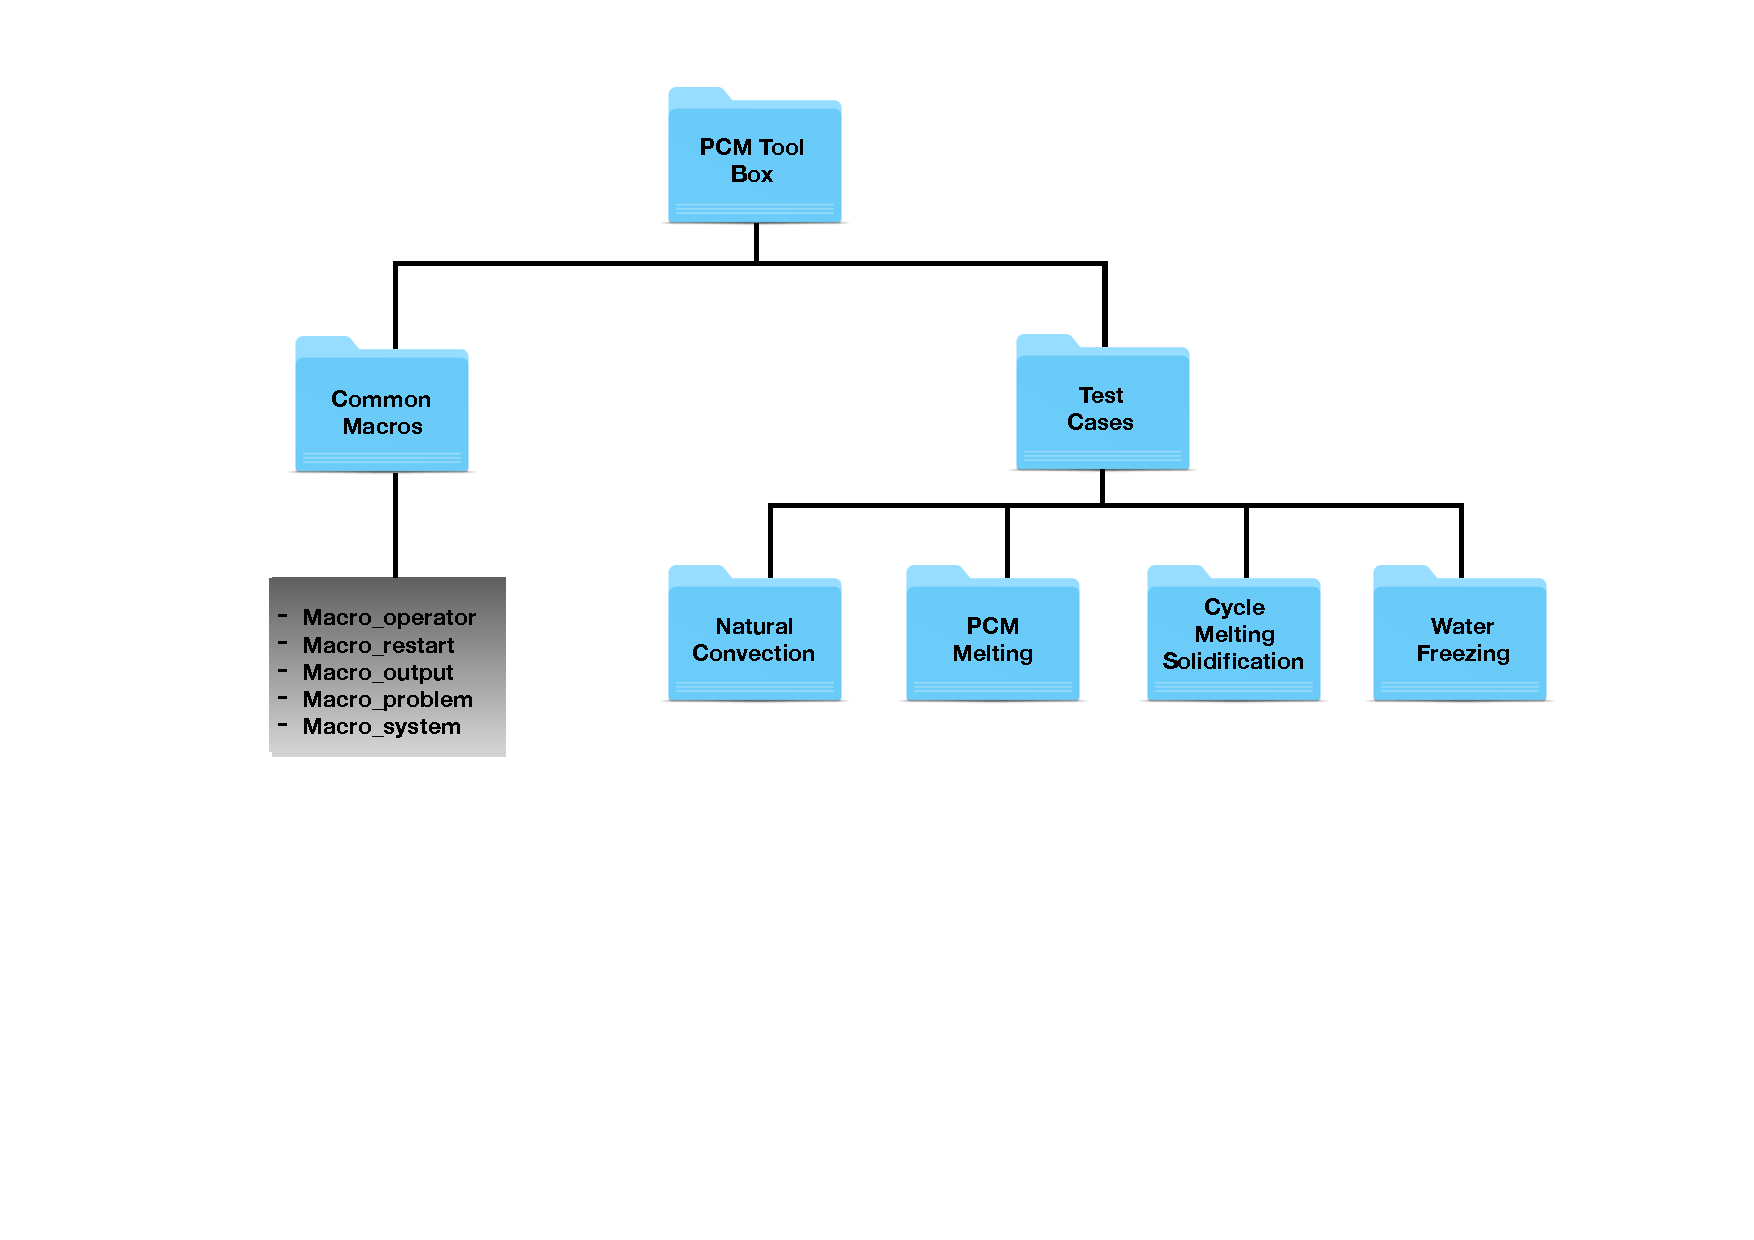
\includegraphics[width=0.9\textwidth]{\figpath/Fig_cap_2/FOLDER_arbor_3}
	\end{center}
	\caption{Folder tree structure of the FreeFem++ toolbox to solve phase change problems. Test cases and common macros are separated into two folders.}
	\label{fig-folder-tree}
\end{figure}

\subsection{Program architecture}
Fig. \ref{fig-folder-tree} gives a schematic overview of the content of the toolbox. All files are provided in a directory called \texttt{PCM-Toolbox}.  Many detailed comments are included in the programs, with direct link to the mathematical expressions used in this chapter. The used \ff syntax was intentionally kept at a low level of technicality and supplemented with detailed comments when specific more technical syntax was used.

\noindent This directory is organized as follows:
\begin{enumerate}
   \item The directory \texttt{Common-Macros} contains five files:\\
$\bullet$ {\em Macro$\_$operator.idp} includes macros and functions defining mathematical operators,\\
$\bullet$ {\em Macro$\_$problem.idp}: macros defining the variational formulation of the problem,\\
$\bullet$ {\em Macro$\_$restart.idp}: macros used to start a new simulation from a saved field,\\
$\bullet$ {\em Macro$\_$output.idp}: macros used to save the solution with different formats,\\
$\bullet$ {\em Macro$\_$system.idp}: macros identifying the OS and defining specific OS-commands.

   \item The directory \texttt{Test-Cases}  contains four subdirectories, each of them defining one of the following applications:\\
    $\bullet$  natural convection of air or water in a differentially heated square cavity, \\
    $\bullet$  melting of a PCM stored in containers of different shapes,\\
    $\bullet$  melting followed by solidification of a rectangular PCM,\\
    $\bullet$  freezing of pure water in a square cavity.
    
   \noindent Each subdirectory contains  three files: {\em NEWTON$\_$\$case.edp} is the main \ff script file, $param_\_phys.inc$ defines the physical parameters and $param_\_num.inc$ the numerical parameters. For example, to run the natural convection case of air in a square cavity, the user can use the following command in a terminal window:
   \begin{lstlisting}
	FreeFem++ NEWTON_stat_natconv.edp
  \end{lstlisting}

  
  \noindent The folder structure of each test case is illustrated in Fig. \ref{fig-case-folder}.
  The obtained solutions are saved in the folder \texttt{OUTPUT/Data}. Depending on the output format selected by the user,  data files are generated in specific folders for being visualized with: Tecplot, Paraview, Gnuplot or Medit. We also provide in the folder \texttt{Figures} ready-made layouts for these visualisation softwares. The user can thus obtain the figures from this paper using  newly generated data. More details about the output structure are given below.
\end{enumerate}

\begin{figure}
	\begin{center}
		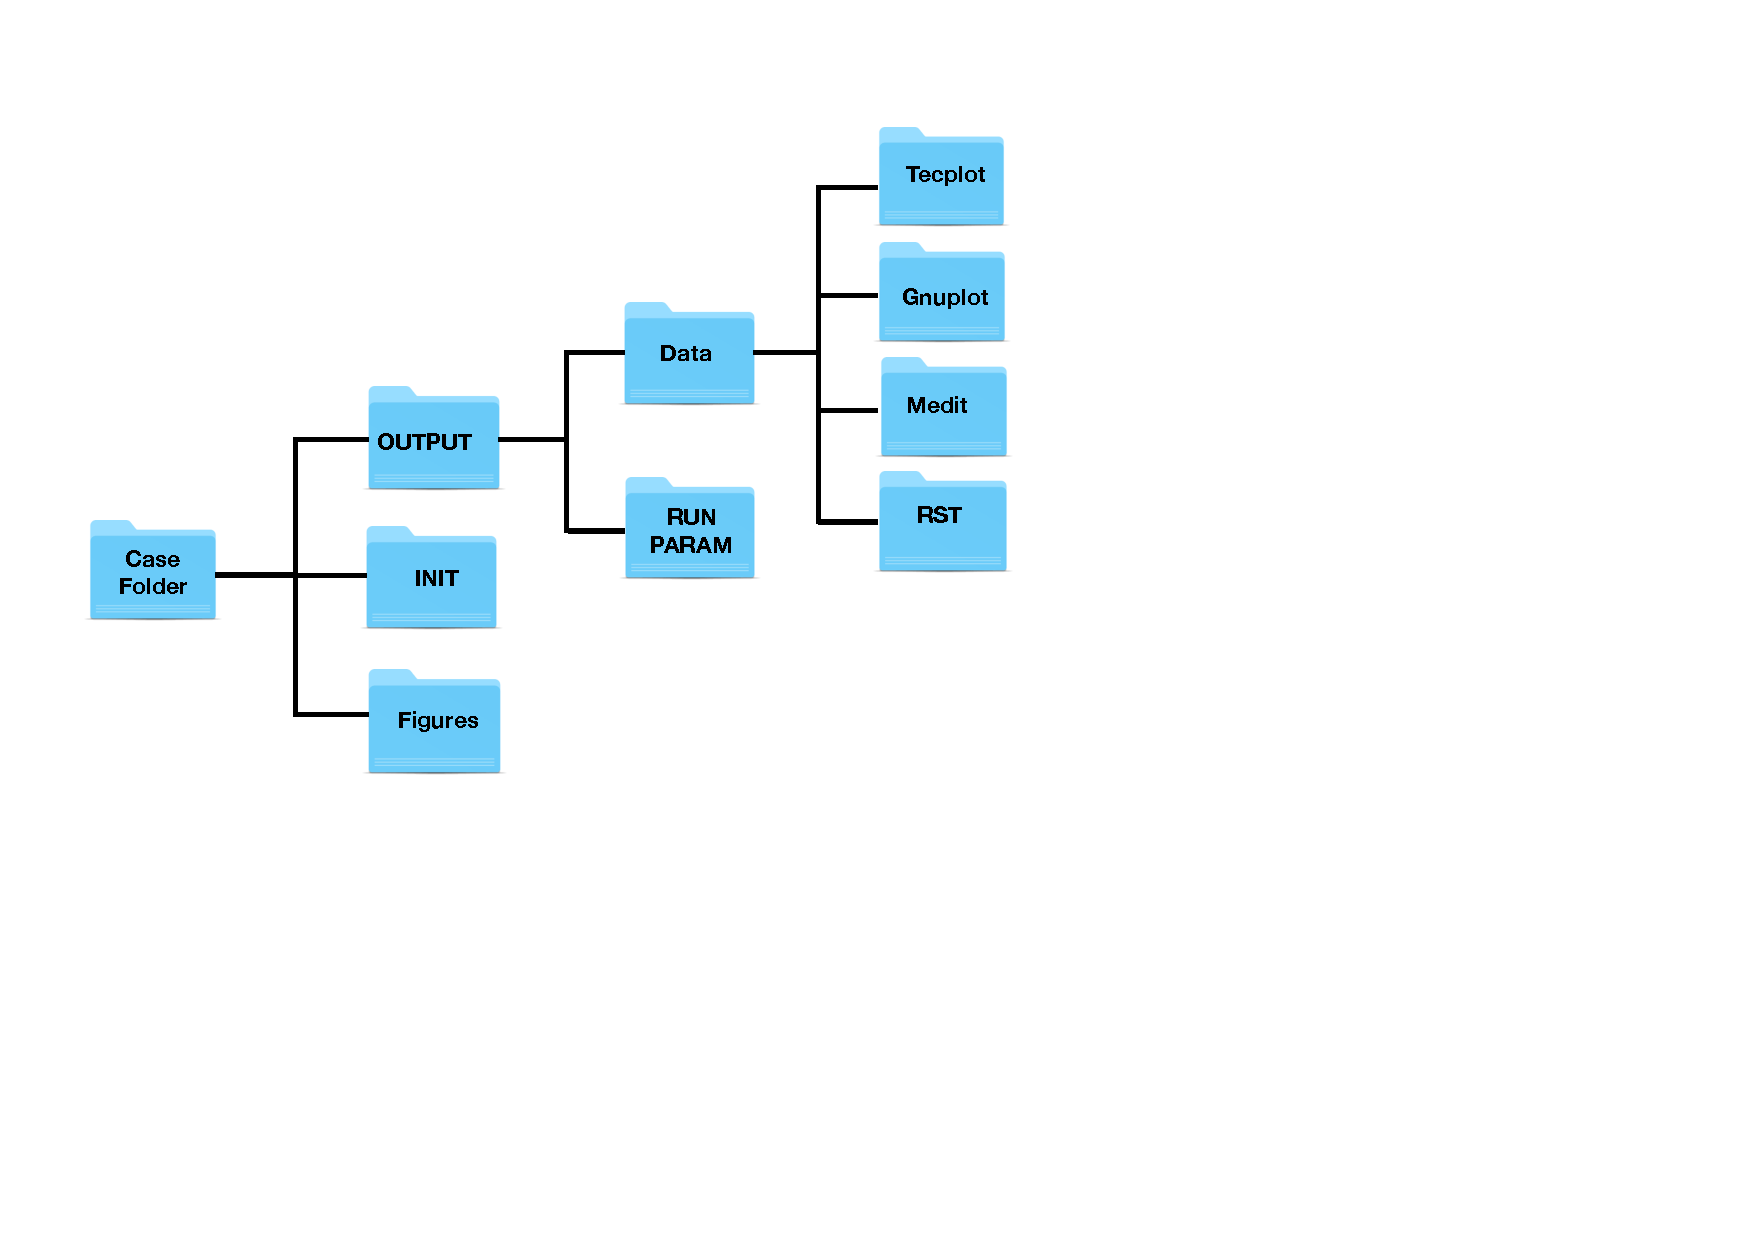
\includegraphics[width=0.8\textwidth]{\figpath/Fig_cap_2/figsCPC_02}
	\end{center}
	\caption{Structure of each Test-case folder. 
	}
	\label{fig-case-folder}
\end{figure}

%\newpage
\subsection{Input parameters}

Physical parameters and parameters related to the run are separated into two files.\\
\textbf{ (1)} The file $param_\_phys.inc$ contains the physical descriptions of the problem:
\begin{itemize}
   \item \textbf{ typeT}: is the finite-element type for the temperature, with possible values \texttt{P2} or \texttt{P1},
   \item \textbf{ Torder}: is the accuracy order of the time integration scheme, with possible values $1$ (Euler scheme) or $2$ (Gear scheme),
   \item \textbf{ scalAdim}: defines the characteristic scales of the problem, see Eq. \ref{eq-adim}. Possible values 1, 2 or 3 correspond to the following choice of the characteristic scales \citep{dan-2014-JCP}:
   \begin{eqnarray} \label{eq-scal1}
    (1) &:&  V_\vref^{(1)} = \frac{\nu_l}{H} \Longrightarrow \ds t_\vref^{(1)} = \frac{H^2}{\nu_l}  \Longrightarrow \Rey=1,\\
      \label{eq-scal2}
     (2) &:& V_\vref^{(2)} = \frac{\alpha}{H} \Longrightarrow \ds t_\vref^{(2)} = t_\vref^{(1)} \Prd  \Longrightarrow \Rey =1/\Prd,\\
      \label{eq-scal3}
     (3) &:& V_\vref^{(3)} = \frac{\nu_l}{H} \sqrt{\frac{\Ray}{\Prd}} \Longrightarrow \ds t_\vref^{(3)} = t_\vref^{(1)} \sqrt{\frac{\Prd}{\Ray}}       \Longrightarrow \Rey = \sqrt{\frac{\Ray}{\Prd}},
\end{eqnarray}

   \item \textbf{ x$_l$, x$_r$, y$_l$, y$_r$}: are the values defining the dimensions of the cavity $[x_l,x_r]\times[y_l,y_r]$,
   \item \textbf{ Pr, Ra, Ste}: are the  Prandtl, Rayleigh and Stefan numbers, see Eq. \ref{eq-Rayleigh} and \ref{eq-RePr},
   \item \textbf{ T$_{hot}$, T$_{cold}$}: are  dimensionless temperatures according to Eq. \ref{eq-adim},
   \item \textbf{ bcu$_1$, bcu$_2$, bcT}: are macros defining the velocity ($\vec u$) and the temperature ($T$) boundary conditions.
   \item \textbf{ epsi}: is the half width $\varepsilon$ of the mushy region. \underline{Default value} = $0.01$,
   \item \textbf{ dt}: is the dimensionless time step,
   \item \textbf{ t$_{max}$}: is the dimensionless final time,
   \item \textbf{ Parameters for regularization functions}: \\
 The parameters of the hyperbolic-tangent function in Eq. \ref{eq-smooth}, used to regularize discontinuous functions are set by default as follows:
 \end{itemize}
    \begin{table}[!ht]
    \centering
    \begin{tabular}{*{8}{c}}
     & { f$_{s}$} & {f$_{l}$} & {a$_s$} & {$\theta_s$} & R$_s$ & {$\CKC$} & {b} \\
       \toprule
       {\textit Enthalpy} & 0 & 1/Ste & 1 & 0.01 & 0.01  & - & - \\
       \midrule
       {\textit Carman - Kozeny} & 0 & 1 & 1 & 0.01 & 0.01  & 10$^6$ & 10$^{-7}$ \\
          \midrule
       {\textit Conductivity (water)} & 1 & 2.26/0.578 & 1 & $\theta_f$ & 0.015 & - & - \\
       \bottomrule
     \end{tabular}
    \label{tab-constant}
    \end{table}
   \begin{itemize} 
    \item \textbf{ rho(T) and Drho(T)}: (water cases only) define  the density and its derivative as functions of the temperature, following the model \citep{Gebhart1977}:\\
 
    \begin{table}[!ht]
    \centering
    \begin{tabular}{*{4}{c}}
    	\multicolumn{4}{c}{
      $\rho(T) = \rho_m (1 - \omega | T - T_m |^q),$}\\	\hline
    $\rho_m$ [kg/m$^3$]  & $\omega$ [$^o$C$^{-q}$] & q & $T_m$  [$^o$C] \\
       \toprule
            $999.972$ & $9.2793 \cdot 10^{-6}$ & $1.894816$ & $4.0293$ \\
       \bottomrule
     \end{tabular}
    \label{tab-rho}
    \end{table}
    \item \textbf{ f$_B$(T), df$_B$(T)}: define the buoyancy force and its derivative.
    \end{itemize}

\noindent \textbf{ (2)} The file {\em param$\_$num.inc} contains the parameters controlling the run.\\
\textbf{ Restart parameters:}
\begin{itemize}
   \item \textbf{ Nsave}: the solution is saved every $N\!save$ time steps in the \texttt{Data} folder (see Fig. \ref{fig-case-folder}). The temperature and the velocity fields are saved in \texttt{Tecplot} and \texttt{Medit} folders, while the liquid fraction, the Nusselt number, and the accumulated heat input are saved in the \texttt{Gnuplot} folder.
   \item \textbf{ Nrestart}: restart files (mesh and solution) are saved every $N\!restart$ time steps. Solutions at current and previous iterations, the CPU time, the accumulated heat input $Q_0$, and the time step $dt$ are saved in the folder \texttt{RST}.
   \item \textbf{ Ncondt}: allows the user to stop the run and save the solution properly. \\
   The file \texttt{OUTPUT/zz.condt} is read every $N\!condt$ time steps: if the user replaces the value "0" in this file by "1" the run is stopped. This is a simple solution for a clean stop of the job by the user. \underline{Default value} = $20$.
   \item \textbf{ Nremesh}: the mesh is adapted every $N\!remesh$ iterations. If this parameter is set to "1" the mesh is adapted every time step.
   \item \textbf{ IFrestart}: is a boolean controlling the set up of the initial field. \\
  $I\!Frestart = 0$, the  initial condition is built in the code for each test case. For the PCM melting cases, the PCM is initially motionless at isothermal temperature. 
  	To set-up a smooth initial field, a few time steps (with very small $\delta t$) are computed by increasing progressively the boundary temperature at the hot wall and the Rayleigh number (by continuation).  Outputs are saved in  \texttt{OUTPUT/Data-RST-0}.\\
   $I\!Frestart > 0$, (positive integer values) the solution field previously computed at iteration $I\!Frestart$ is loaded from the folder \texttt{OUTPUT/Data-RST-filenameRST/RST}, \\
   with \texttt{filenameRST} a variable selecting the restart folder. \\
   $I\!Frestart < 0$, (negative integer values), the same principle for loading a solution is used, but from the folder \texttt{INIT}  (see Fig. \ref{fig-case-folder}). The solution fields stored in this folder could come from different previous calculations (\eg a steady state solution or, for the water, the natural convection field before freezing).
\end{itemize}

\noindent \textbf{ Newton parameters:}
\begin{itemize}
   \item \textbf{ epsconv}: is the value of  the stopping criterion for steady cases,
   \item \textbf{ gamma}: is the penalty parameter in Eq. \ref{eq-time-disc1}. \underline{Default value} = $10^{-7}$,
   \item \textbf{ tolNewton}: is the Newton tolerance $\xi_N$ (see Eq. \ref{eq-Newton-algo}). \underline{Default value} = $10^{-6}$,
   \item \textbf{ newtonMax}: limits the maximum number of iterations in  the Newton algorithm (Eq. \ref{eq-Newton-algo}). \\
   \underline{Default value} = $50$,
  % \Blue{\textit {\textbf c$_1$, c$_2$, c$_3$}: \Red{(-- why not negative $a_2$ ?? si c'est trop compliqu� de changer, il faut le laisser tel quel --$>$ } \Blue{C'est modifi� en a$_2$ n�gatif maintenant dans le code)--}  are the coefficients of the time integration scheme: c$_1 =1/$dt, c$_2 = -1/$dt, c$_3 = 0$ correspond to the first order backward Euler scheme and c$_1 =1.5/$dt, c$_2 = -2/$dt, and c$_3 = 0.5/$dt to the second order Gear scheme.}
\end{itemize}

\noindent \textbf{ Mesh parameters:}
\begin{itemize}
   \item \textbf{ nbseg}: is  the number of segments for the discretisation along the $x$ and $y$ directions,
   \item \textbf{ errh}: is the interpolation error level. \underline{Default value} = $0.02$,
   \item \textbf{ hmin, hmax}: are the minimum and maximum edge size, respectively,
   \item \textbf{ adaptratio}: is the ratio for a prescribed smoothing of the metric. For a value less than $1.1$ no smoothing is done. \underline{Default value} = $1.5$,
   \item \textbf{ nbvx}: is the maximum number of vertices allowed in the mesh generator. \underline{Default value} = $50000$.
\end{itemize}

\noindent \textbf{ Output parameters:}
   \begin{itemize}
      \item \textbf{ dircase}: is the name of the output folder,
      \item \textbf{ fcase}: is the prefix-name for ouput files.
      \item \textbf{ Tecplot, Medit, Gnu}: correspond to the name of the visualisation software to be used; the format of the outputs written in \texttt{OUTPUT/Data} (see Fig. \ref{fig-case-folder}) is accordingly set.  The files from the Tecplot folder can be easily read  also with Paraview.
   \end{itemize}
   
\subsection{Outputs}
When a computation starts, the \texttt{OUTPUT} directory is created (see Fig. \ref{fig-case-folder}).
It contains two folders storing the output data and the echo of the run parameters.
The folder \texttt{Data} contains four subdirectories with different output format files of the computed solution. File names are created using  the prefix defined by the parameter \textbf{ fcase}, the current iteration and the current dimensionless time $t$. 
Solution files can be visualized using either Tecplot or any other CFD Visualization tools (Paraview, Visit, etc.). 
Moreover, {\em .gmsh}  (mesh) and {\em .rst} (fields) files are generated in the folder \texttt{RST} to enable restarts of the computation. Note that the folder \texttt{FFglut} contains  \ff scripts that re-read and visualize the RST-files to facilitate the selection of a restart field.  
An {\em .echo} file with a summary of the main parameters, informations on the run and the names of the output files is saved in the folder \texttt{RUNPARAM}.  This directory additionally contains a copy of the {\em .inc} parameter files, allowing an easy identification of each case and preparing an eventual rerun of the same case.


\section{Numerical tests of the accuracy of the numerical method}\label{sec-numconv}

We start by presenting tests of the accuracy of our numerical method. We used the technique of manufactured solutions (\eg \cite{BEC-book-1998-Roache}) which has the advantage of providing an exact solution to a modified problem, related to the initial one.  The general idea is to modify the
original system of equations by introducing an extra source term, such that the new system admits an exact solution
given by a convenient analytic expression. Even though in most cases exact solutions constructed in this way are not physically realistic,
this approach allows one to rigorously verify computations.\\
We tested the space and time accuracy using manufactured solutions for the system of Eqs. \ref{eq-qmvt} - \ref{eq-energ} for a stationary case (Burggraf flow) and a time-dependent one \citep{nourgaliev2016fully}. For both cases, we computed the global error $ \varepsilon$ for different norms in space:
\begin{equation}
  \varepsilon  = \| \Phi_e - \phi_h \|,
  \label{eq-epsconv}
\end{equation}
with $\Phi_e$ the exact solution and $\phi_h$ the numerical solution. Computations were performed for the convection of air ($C=K=1$, $A(\theta)=S(\theta)=0$), with a Rayleigh number $\Ray = 10^4$ and a Prandtl number $\Prd = 0.71$.


%%%%%%%%%%%%%%%%%%%%%%%%%%%%%%%%%%%%%%%%%%%%
\subsection{Space accuracy: Burggraf stationary flow with thermal effects} \label{subsub-conv-burg}

The Burggraf manufactured solution  is a time-independent recirculating flow inside a square cavity $[ 0 , 1] \times [ 0 , 1]$. It is similar to the well-known  entrained cavity flow, with the difference that the velocity singularity at the top corners of the cavity is avoided. We added to the classical Burggraf flow \citep{Shih-1989,Lamballais-2009} a manufactured solution for the temperature, with 
constant temperature imposed at the top and the bottom walls. Vertical walls are assumed to be adiabatic.
The exact solution of the new flow with thermal effects is:
\begin{eqnarray}
\label{burggraf-u}
   u_1(x,y) &=& \sigma g'(x) h'(y), \\\nonumber
   u_2(x,y) &=& - \sigma g''(x) h(y), \\\nonumber
   p(x,y)   &=& \frac{\sigma}{\Rey} \left( h^{(3)}(y) g(x) + g''(x)h'(y) \right) + \frac{\sigma^2}{2} g'(x)^2 \left( h(y)h''(y)-h'(y)^2 \right),\\ \nonumber
   T(x,y) &=& T_{c} + (T_{h} - T_{c}) y + a(x) b(y), 
\end{eqnarray}
with $\sigma >0$ a scaling parameter and functions
\begin{eqnarray}
   g(x) &=& \frac{x^5}{5} - \frac{x^4}{2} + \frac{x^3}{3}, \\ \nonumber
   h(y) &=& y^4 - y^2, \\ \nonumber
   a(x) &=& \cos (\pi x), \\ \nonumber
   b(x) &=& y(1-y).
\end{eqnarray}
Note that  the velocity at the top border of the cavity is:
\begin{equation}
u_1(0,1) = 2\sigma (x^4 - 2x^3 + x^2), \quad u_2(x,1) =0,
\end{equation}
which ensures the continuity of the velocity at the corners ($\vec{u}(0,1) =\vec{u}(1,1) =0$), since no-slip walls are imposed for the other borders:
$\vec{u}(x,0) = \vec{u}(0,y) = \vec{u}(1,y) = 0$. 




The forcing terms that have to be added to the momentum and energy (temperature) equation are derived by injecting the exact solution \ref{burggraf-u} into the system of Eqs. \ref{eq-qmvt} - \ref{eq-energ}:
\begin{eqnarray}
   f_{u_1} &=& 0, \\ \nonumber
   f_{u_2} &=& \sigma^2 h(y) h'(y) \left( g''(x)^2 - g'(x)g^{(3)}(x) \right) \\ \nonumber
   &+& \frac{\sigma}{\Rey}\left( g^{(4)}(x) h(y) + 2 g''(x)h''(y) + g(x) h^{(4)}(y) \right) \\ \nonumber
   &+& \frac{\sigma^2}{2} g'(x)^2 \left( h(y) h^{(3)}(y) - h'(y)h''(y) \right) - \frac{\Ray}{\Prd \Rey^2} T(x,y),\\ \nonumber
   f_T &=& u_1(x,y) a'(x) b(y) + u_2(x,y) \left( T_h - T_c + a(x) b'(y) \right) \\ \nonumber
   &-& \frac{K}{\Rey \Prd} \left( a''(x)b(y) + a(x) b''(y) \right).
\end{eqnarray}
We used the Taylor-Hood finite element ($\PP_2$ for the velocity and $\PP_1$ for the pressure)  and tested $\PP_1$ or $\PP_2$ finite elements for the temperature.
Figs. \ref{fig-conv-burggraf}a and  \ref{fig-conv-burggraf}b illustrate the streamlines and the temperature field, respectively.
Fig. \ref{fig-conv-burggraf} plots the  discretization error $\varepsilon$  as a function of the grid size $h=\delta x=\delta y$ for the temperature.  Both ${L}^2$ and ${L}^\infty$ norms are displayed. The expected second order accuracy in  ${L}^2$-norm is obtained with  $\PP_1$ finite elements (Fig. \ref{fig-conv-burggraf}c), while an order exceeding three is 
observed when  $\PP_2$ finite elements are used (Fig. \ref{fig-conv-burggraf}d).
\begin{figure}[!ht]
	\begin{center}
		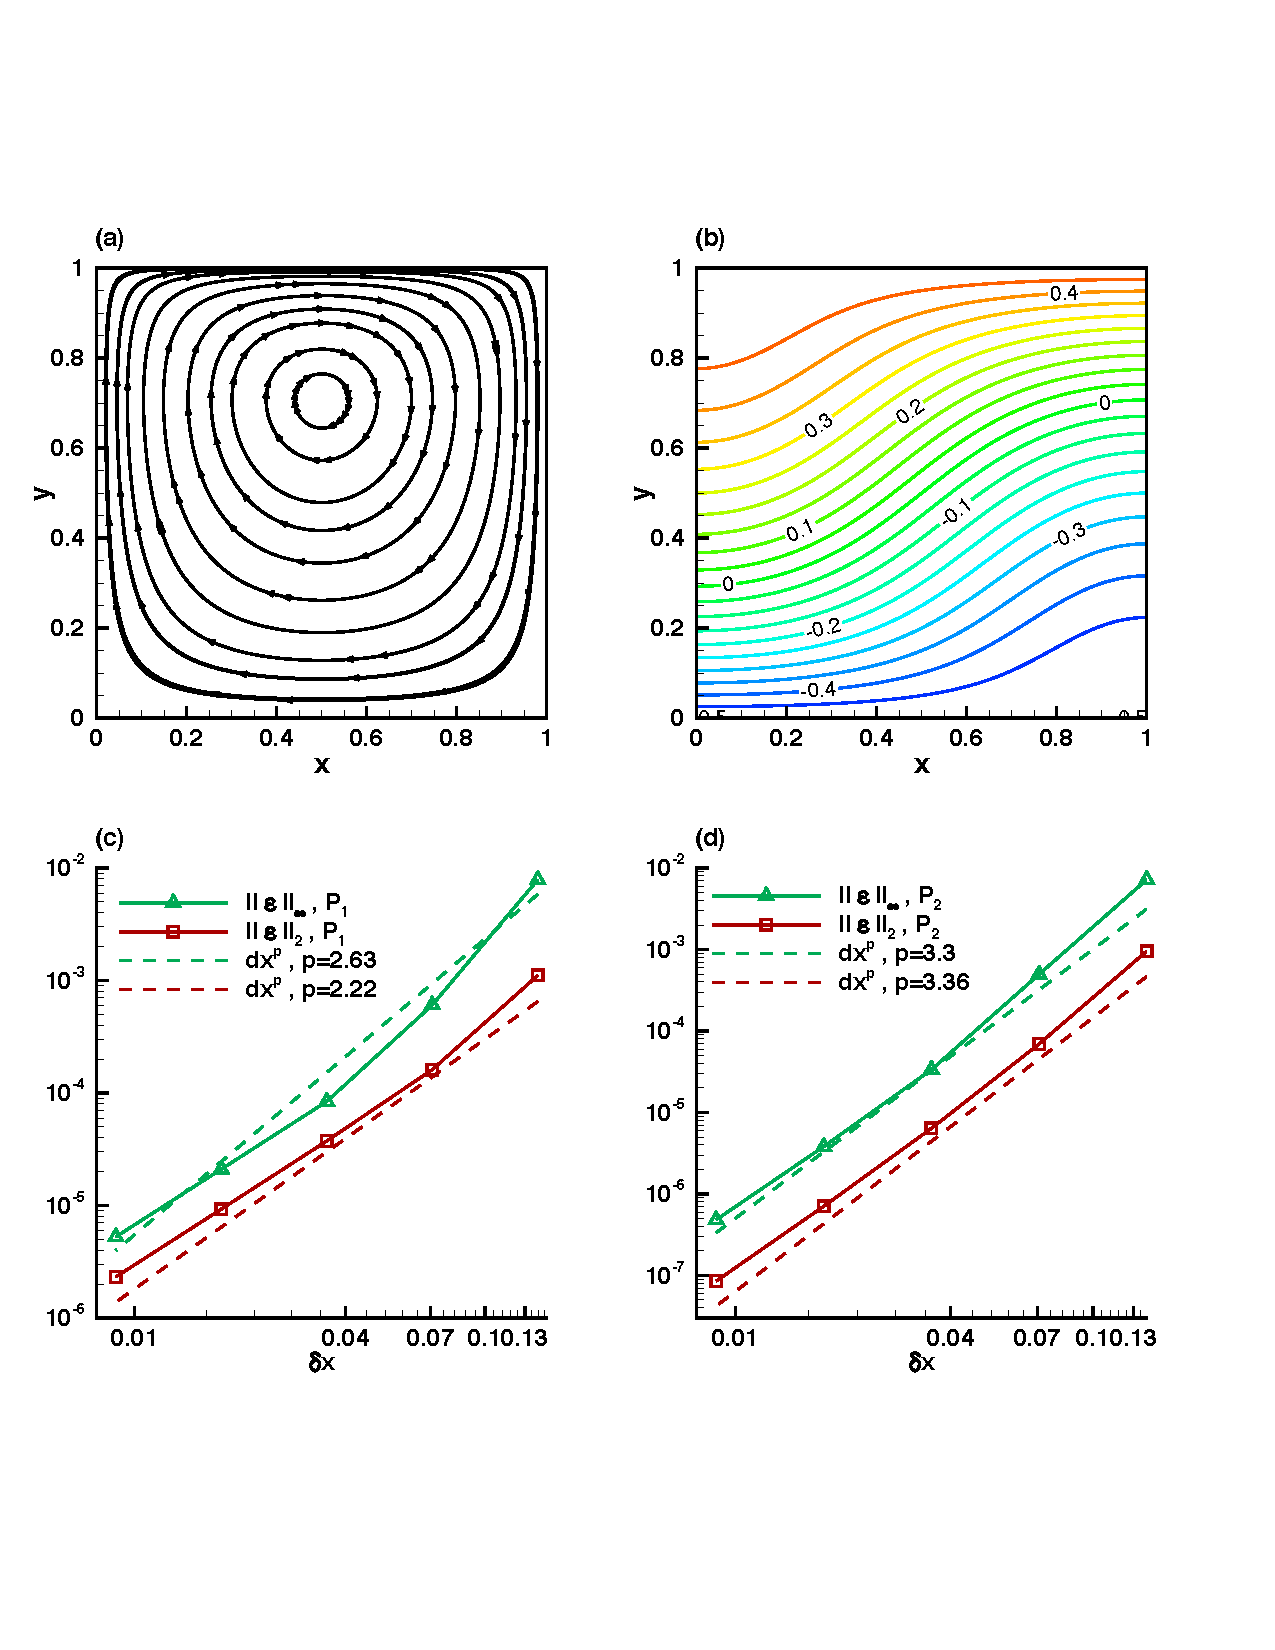
\includegraphics[width=\textwidth]{\figpath/Fig_cap_2/figsCPC_03} 
	\end{center}
	\caption{Burggraf stationary flow with thermal effects used to test the space accuracy of the numerical scheme. Streamlines (a) and temperature contours (b) of the flow field.	
Global error $\varepsilon$ (cf. Eq. \ref{eq-epsconv}) for  the temperature: (c) $\PP_1$ and (d) $\PP_2$ finite elements.}
	\label{fig-conv-burggraf}
\end{figure}

%\pagebreak
%%%%%%%%%%%%%%%%%%%%%%%%%%%%%%%%%%%%%%%%%%%
\subsection{Time accuracy: manufactured unsteady solution} \label{subsub-conv-nourg}

To test the time accuracy of the Gear (BDF2) scheme, we used the manufactured time-dependent solution suggested in \cite{nourgaliev2016fully}:
\begin{align}
\label{eq-manufN}
	u_1(x,y,t) &=& \left( \delta U_0 + \alpha_u \, \sin(t) \right) \, \cos(x+ \gamma_1 t) \, \sin(y+ \gamma_2 t), \\ \nonumber
	u_2(x,y,t) &=& - \left( \delta U_0 + \alpha_u \sin(t) \right) \, \sin(x+ \gamma_1 t) \, \cos(y+ \gamma_2 t), \\ \nonumber
	T(x,y,t) &=& \bar{T} + \left( \delta T_0 + \alpha_t \sin(t) \right) \, \cos(x+ \gamma_1 t) \, \sin(y+ \gamma_2 t), \\ \nonumber
	p(x,y,t) &=& \bar{P} + \left(\delta P_0 + \alpha_p \sin(t) \right) \, \sin(x+ \gamma_1 t) \, \cos(y+ \gamma_2 t), 
\end{align}
The values of the constants are reported in Table \ref{tab-const-Nourga}.
\begin{table}[!ht]
\centering
\begin{tabular}{*{10}{c}}
 % \toprule
  $\gamma_1$ & $\gamma_2$ & $\bar{P}$ & $\bar{T}$ & $\delta P_0$ & $\delta T_0$ & $\delta U_0$ & $\alpha_p$ & $\alpha_u$ & $\alpha_t$\\
   \midrule
  $0.1$ & $0.1$ & $0$ & $1.0$ &  $0.1$ & $1.0$ & $1.0$ & $0.05$ & $0.4$ & $0.1$ \\
 % \bottomrule
 \end{tabular}
\caption{Parameter for the time-dependent manufactured solution (\ref{eq-manufN}).}
\label{tab-const-Nourga}
\end{table}

\noindent The corresponding forcing source terms are
\begin{eqnarray}
	f_{u_1} &=& \alpha_u \, \cos(t) \, \cos(a) \sin(b) - U_c \, \gamma_1 \, \sin(a) \sin(b) + U_c \, \gamma_2  \, \cos(a)\cos(b) \\ \nonumber
	  & & - U_c \,  u_1(x,y,t) \, \sin(a) \sin(b) + U_c \,  u_2(x,y,t) \, \cos(a) \cos(b)
	  + P_c \, \cos(a) \cos(b)\\ \nonumber
	  & & + \frac{2}{\Rey} \, u_1(x,y,t), \\	  \nonumber
	f_{u_2} &=& - \alpha_u \,  \cos(t)  \, \sin(a) \cos(b) - U_c \,  \gamma_1  \,  \cos(a) \cos(b) + U_c \,  \gamma_2 \,  \sin(a)\sin(b) \\ \nonumber
		  & & - U_c \,  u_1(x,y,t)  \,  \cos(a) \cos(b) + U_c  \, u_2(x,y,t)  \,  \sin(a) \sin(b)
		  -  P_c  \,  \sin(a)  \,  \sin(b)\\ \nonumber
		  & &+ \frac{2}{\Rey} \,  u_2(x,y,t)
		  - \frac{\Ray}{\Prd \Rey^2} \,  T(x,y,t), \\  \nonumber
	f_{T} &=& \alpha_t \,  \cos(t) \,  \cos(a) \sin(b) -  T_c  \,  \gamma_1 \,  \sin(a) \sin(b) + T_c \,   \gamma_2  \,  \cos(a)\cos(b) \\ \nonumber
		  & &-  T_c \,  u_1(x,y,t)  \,  \sin(a) \sin(b)  
		  +   T_c  \,  u_2(x,y,t)  \, \cos(a) \cos(b) 
		  + \frac{2 K}{\Rey \Prd} \,  T_c  \, \cos(a) \sin(b), \\ \nonumber
\end{eqnarray}
where $a = (x+ \gamma_1 t), \,
b = (y+ \gamma_2 t)$ and  
$U_c = (\delta U_0 + \alpha_u \sin(t)), \,
	T_c = (\delta T_0 + \alpha_u \sin(t)), \,
	P_c = (\delta P_0 + \alpha_u \sin(t))$.

Guided by  the results obtained  in Sec. \ref{subsub-conv-burg} for the space accuracy, we fixed the grid size to $h=dx = 0.01$ to ensure small spatial discretization errors.
For diminishing values of the time step $\delta t$, the solution was evolved in time up to the time instant $t_{max} = \pi$ at which the error Eq. \ref{eq-epsconv} was computed. 
The time convergence is displayed in Fig. \ref{fig-conv-bdf2} for the temperature variable. 
The expected second order convergence in time is obtained for both $\PP_1$ (Fig. \ref{fig-conv-bdf2}a) and $\PP_2$ (Fig. \ref{fig-conv-bdf2}b) discretizations of the temperature.

\begin{figure}[!ht]
	\begin{center}
		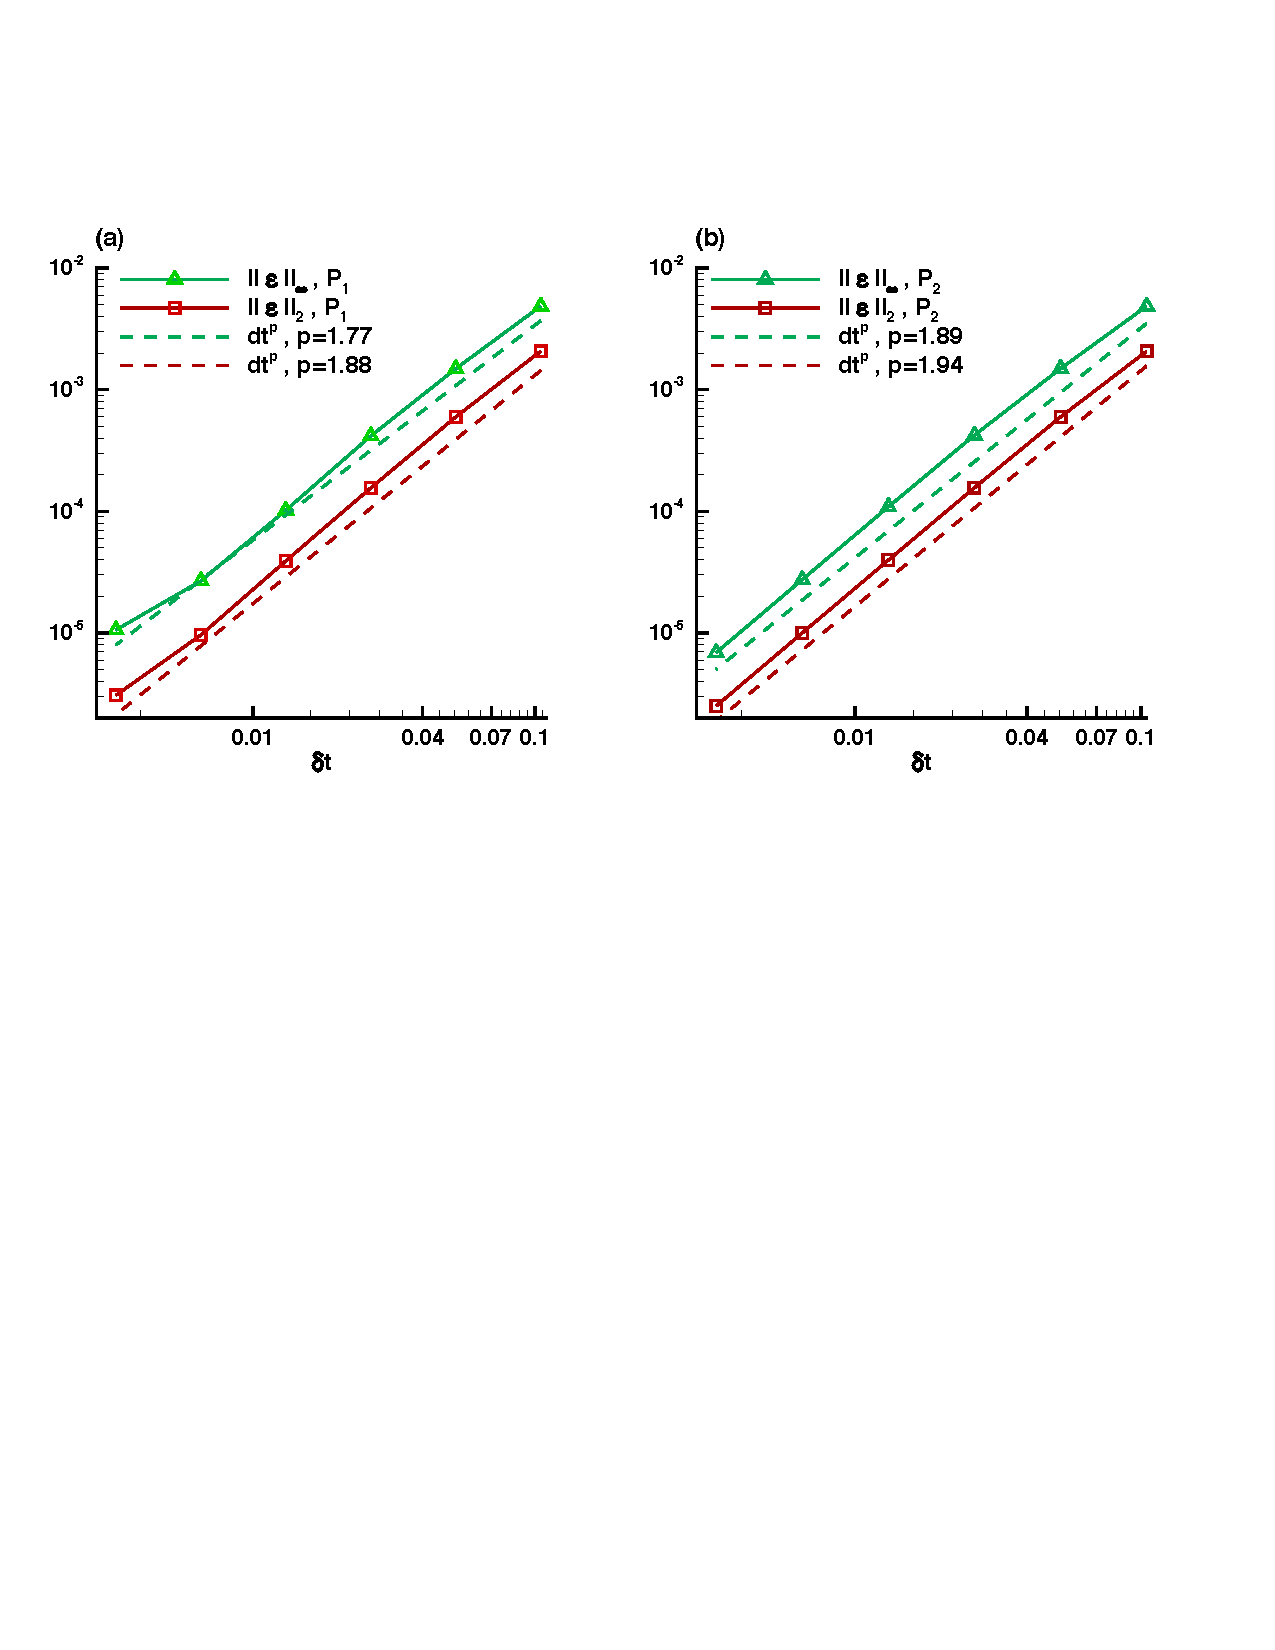
\includegraphics[width=\textwidth]{\figpath/Fig_cap_2/figsCPC_04} 
	\end{center}
	\caption{Time accuracy of the numerical scheme tested using the time-dependent manufactured solution of \cite{nourgaliev2016fully}. Evolution of the global error $\varepsilon$ given in Eq. \ref{eq-epsconv} for  the temperature at $t_{max} = \pi$. Discretizations using: (a) $\PP_1$ and (b) $\PP_2$finite elements.}
	\label{fig-conv-bdf2}
\end{figure}

\newpage
\section{Domain decomposition method with FreeFem++: FFDDM}
Solving the Navier-Stokes-Boussinesq systems of Eqs. \ref{eq-weak-all} - \ref{eq-weak-energy} in three-dimensional configurations could generate a large problem size.
The natural convection of air in a cube of dimensions $[0,1]^3$ with $40 \times 40 \times 40$ uniform grids involves indeed $3$ millions of unknowns (d.o.f.) in the linear system, when a $\PP_1$ finite element is considered for the temperature.
For such a large size of problem, memory lack issue can rapidly arise with sequential algorithms.
It is thus essential to distribute data among several processors.

A natural approach is the domain decomposition method (DDM).
DDM aims at dividing the computational domain in many subdomains on which we solve local problems with the adequate interface conditions.
Two families of DDM exists: non-overlapping methods and overlapping methods such as Schwarz method.

\noindent We perform in this work a domain decomposition Schwarz method, enhanced by coarse space corrections through the \ff library \texttt{ffddm}.
This enrichment with coarse space is mandatory in the present study to avoid the lack of robustness related to the One-Level method. 
It is well-known indeed that the main drawback of such One-Level methods is their convergence rate that depends on the number of subdomains,
resulting to a poor scale for large problems. 
This is mostly due to a lack of global communication between subdomains that exchanges informations with its direct neighbors only.
The additional coarse space has consequently the task to spread the informations to all subdomains at each iteration.

%We use the recent library \texttt{ffddm} that makes available in \ff state-of-the-art scalable Schwarz domain decomposition methods (DDM).
%FFDDM (FreeFem++ Domain Decomposition Method) is a parallel part of FreeFem++ allowing to use parallel solver in FreeFem++.
 %The DDM approach is based on a Schwarz method enhanced by coarse space corrections.
%The data distribution among the processor is done via an overlapping domain decomposition and a related linear algebra.
%The linear system is then solved by using the domain decomposition method as preconditioners to the GMRES Krylov method.

The data distribution among the processor is done via an overlapping domain decomposition and a related linear algebra.
To enable parallel computing, the mesh is first split into subdomains using \texttt{Scotch} or \texttt{Metis} libraries. 
Fig. \ref{fig:mesh-partition} illustrates the domain decomposition of a cube of dimensions $[0,1]^3$ into $8$ subdomains with \texttt{Metis} graph partitioner. 
Mesh adaptivity using metrics control makes possible the optimisation of the distribution of mesh elements.
%Then, a  domain decomposition Schwarz method, enhanced by coarse space corrections, is used through the \ff library \texttt{ffddm}. 


\begin{figure}
	\begin{center}
		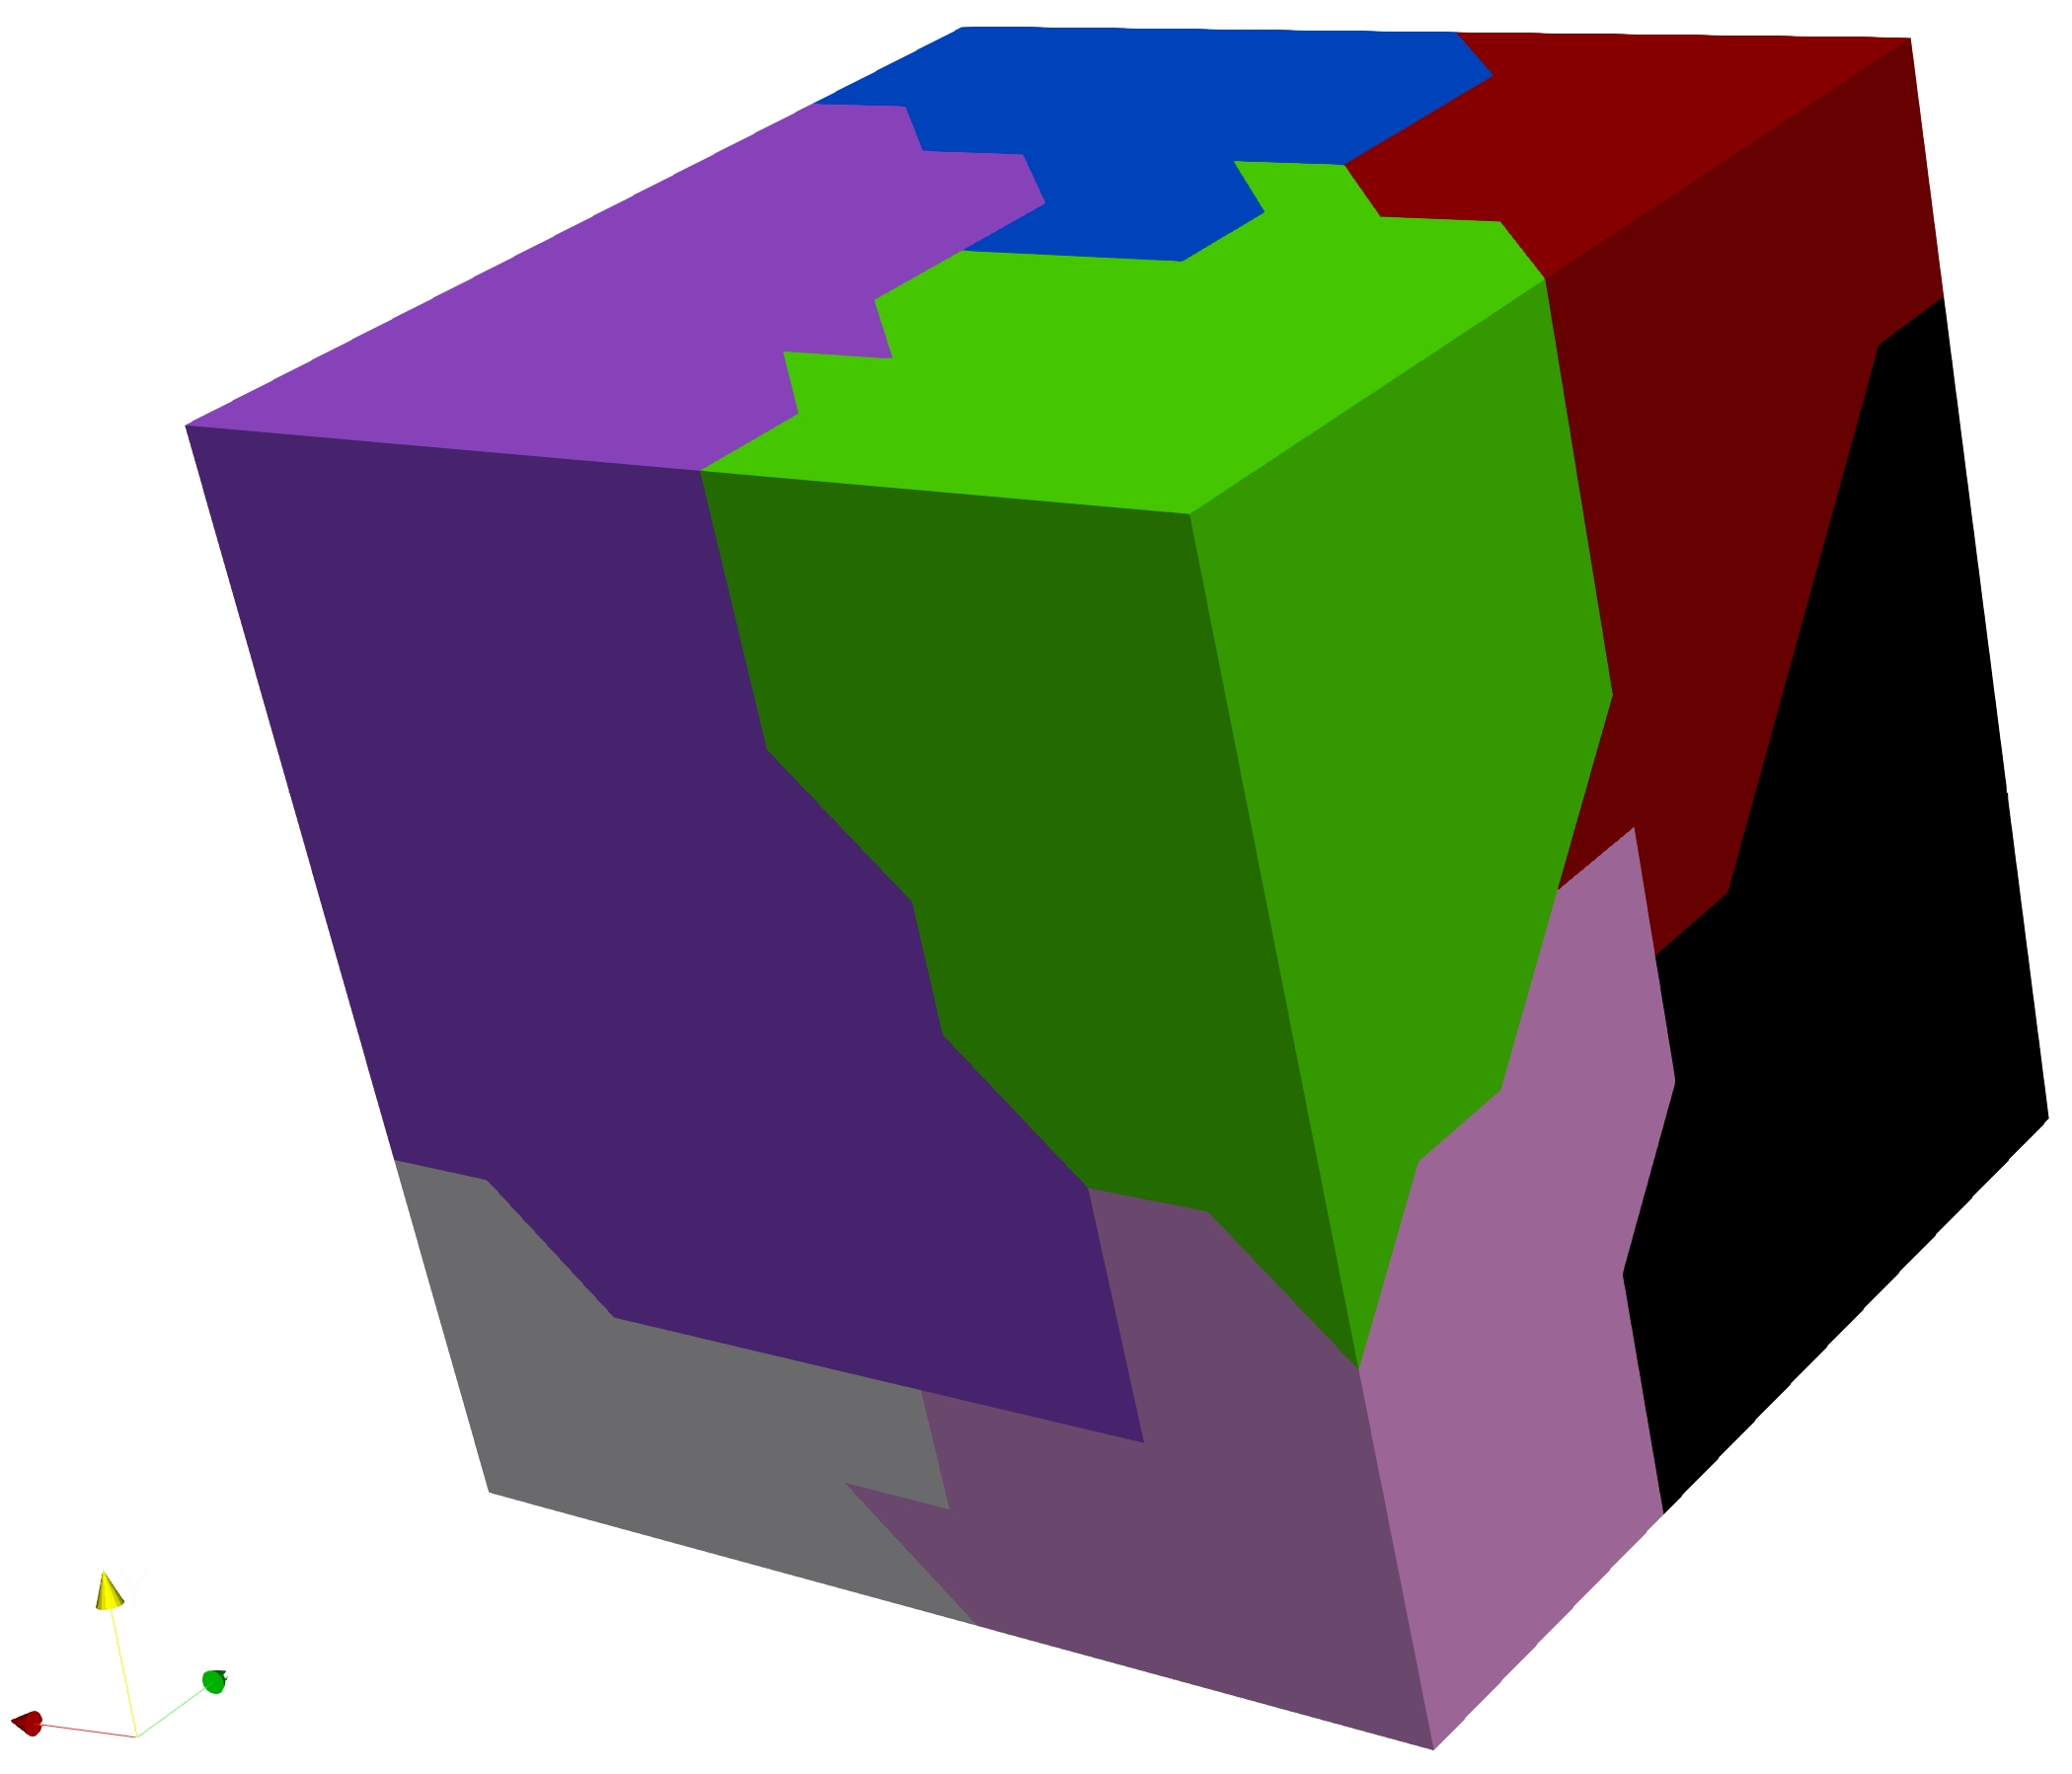
\includegraphics[width=.5\textwidth]{\figpath/Fig_cap_meth-num/Partitionning}
	\end{center}
	\caption{Partition of $\Omega = [0,1]^3 $ into $8$ subdomains with \texttt{Metis} partitioner.}
	\label{fig:mesh-partition}
\end{figure}

\noindent The  final linear system of Eqs. \ref{eq-newton-C1} - \ref{eq-newton-C3} is solved in parallel using a GMRES Krylov method, with an Optimized Restricted Additive Schwarz (ORAS) preconditioner.  
To solve the linear equation $A x = rhs$, the ORAS preconditionner reads
\begin{equation}
   M_{RAS}^{-1} = \sum_{j=1}^{\mathcal{N}} R^T_j D_j (R_j A R^T_j)^{-1} R_j,
\end{equation}

\noindent $R_j$ denote the restriction operators and $D_j$ are square diagonal matrices.
Local matrices are defined as:
\begin{equation}
   A_j = R_i A R_i^T.
\end{equation}

\noindent The duplicated unknowns due to the overlap between subdomains are coupled via a partition of unity
\begin{equation}
   I = \sum_{i=1}^{\mathcal{N}} R_i^T D_i R_i.
\end{equation}

\noindent Thus, the global solution $U$ is defined as:
\begin{equation}
  U = \sum_{i=1}^{\mathcal{N}} R_i^T D_i R_i U =  \sum_{i=1}^{\mathcal{N}} R_i^T D_i U_i.
\end{equation}

We assess the strong scalability of the ORAS preconditioner on the 3D differentially heated cube cavity.
We vary the number of subdomains while the global system size is fixed.
With a $\PP_2$ finite element for the temperature, we solve $7.2$ million of unknowns (d.o.f).
The subdomain is decomposed into subdomains with \texttt{Metis}, ranging from $48$ to $400$ subdomains.
Fig. \ref{fig-scalability} illustrates the evolution of the total wall clock time for different subdomains, in which a good speed up is observed.
From $48$ to $320$ we observe a linear speed up. 
The total runtime passes from $2$ hours for $48$ subdomains to $15$ minutes for $320$ subdomains.
The linear speed up is then slightly lost for $400$ subdomains but remains reasonable.
In Tab. \ref{tab-scalability} we detail the timing relative to this test.
The column "Factorization" denotes the time spent in the factorization of the local submatrices and "GMRES" gives the time taken by GMRES to solve the global linear system
by the domain decomposition algorithm.

\begin{figure}%[!htbp]
\begin{minipage}{\linewidth}
\begin{center}
 {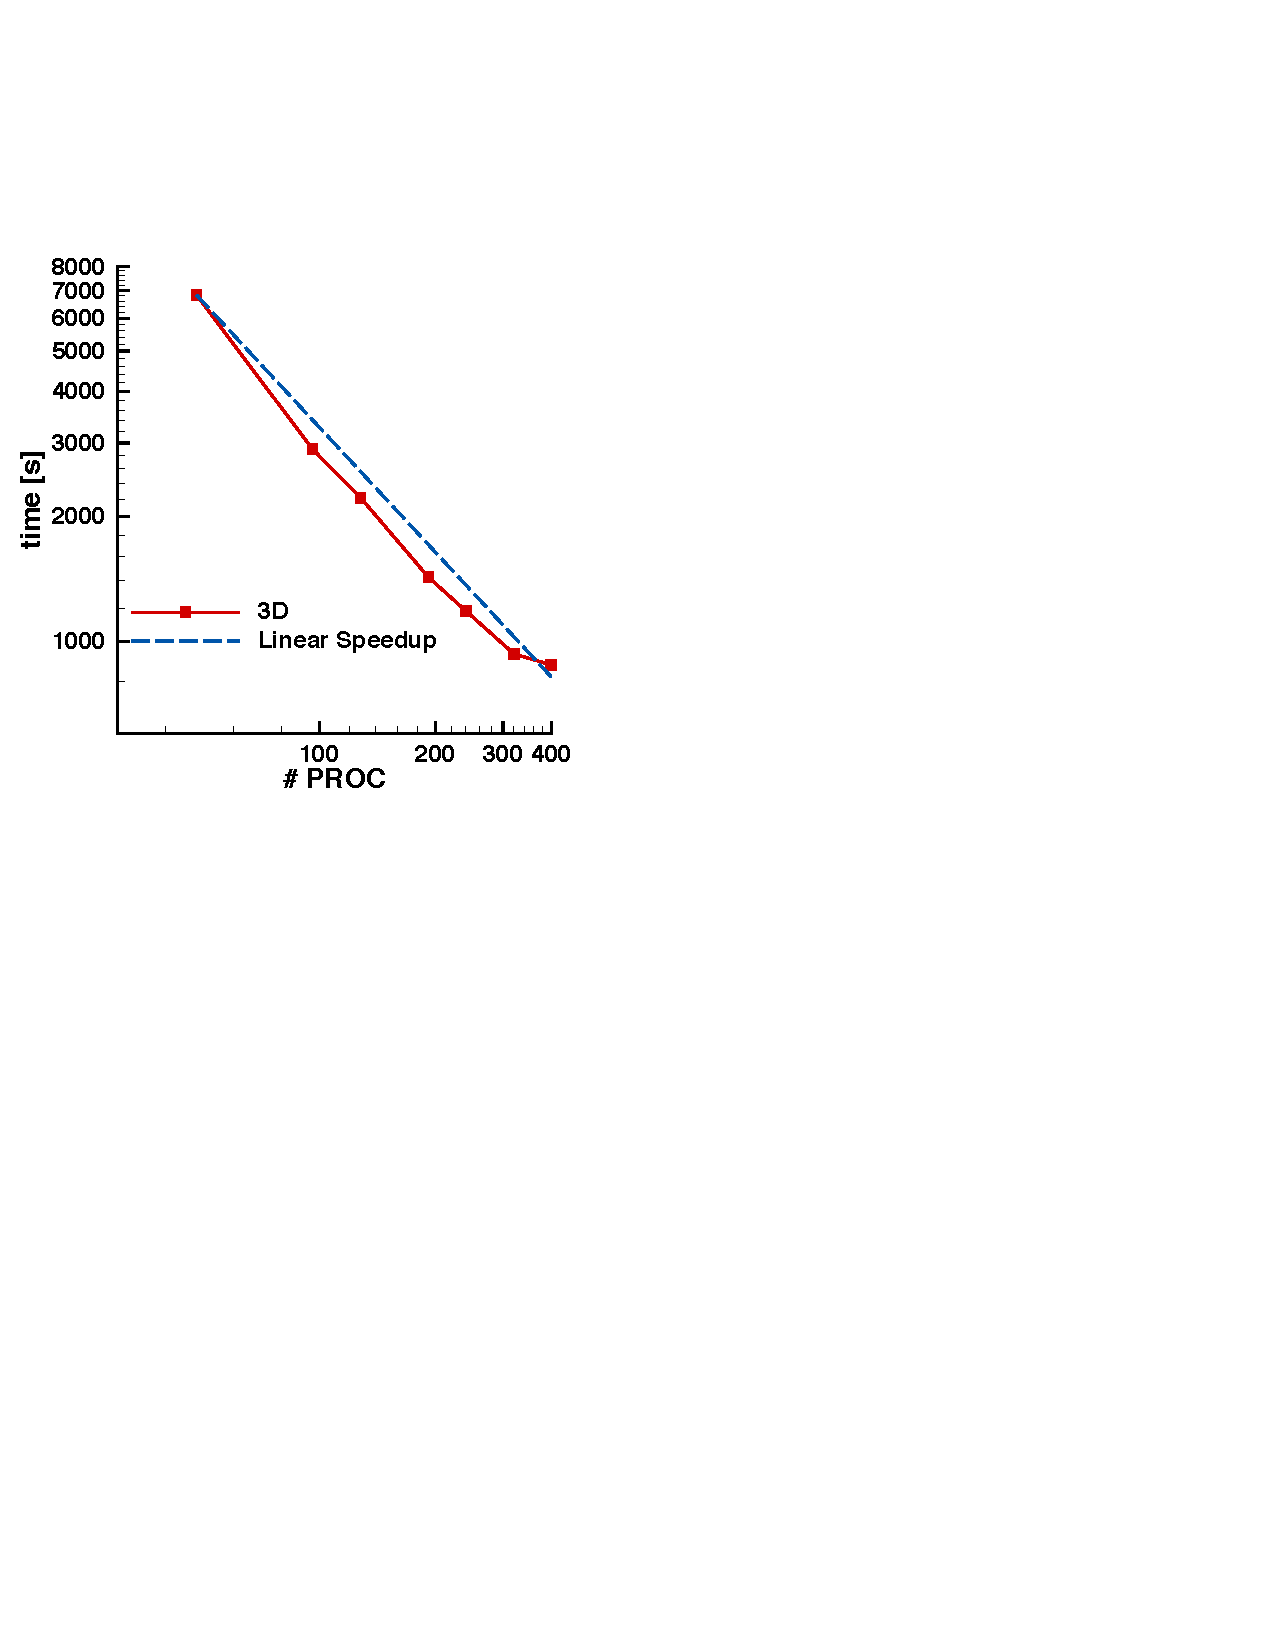
\includegraphics[width=.49\textwidth]{\figpath/Fig_cap_natconv/Scal_ffddm_2level}}
 {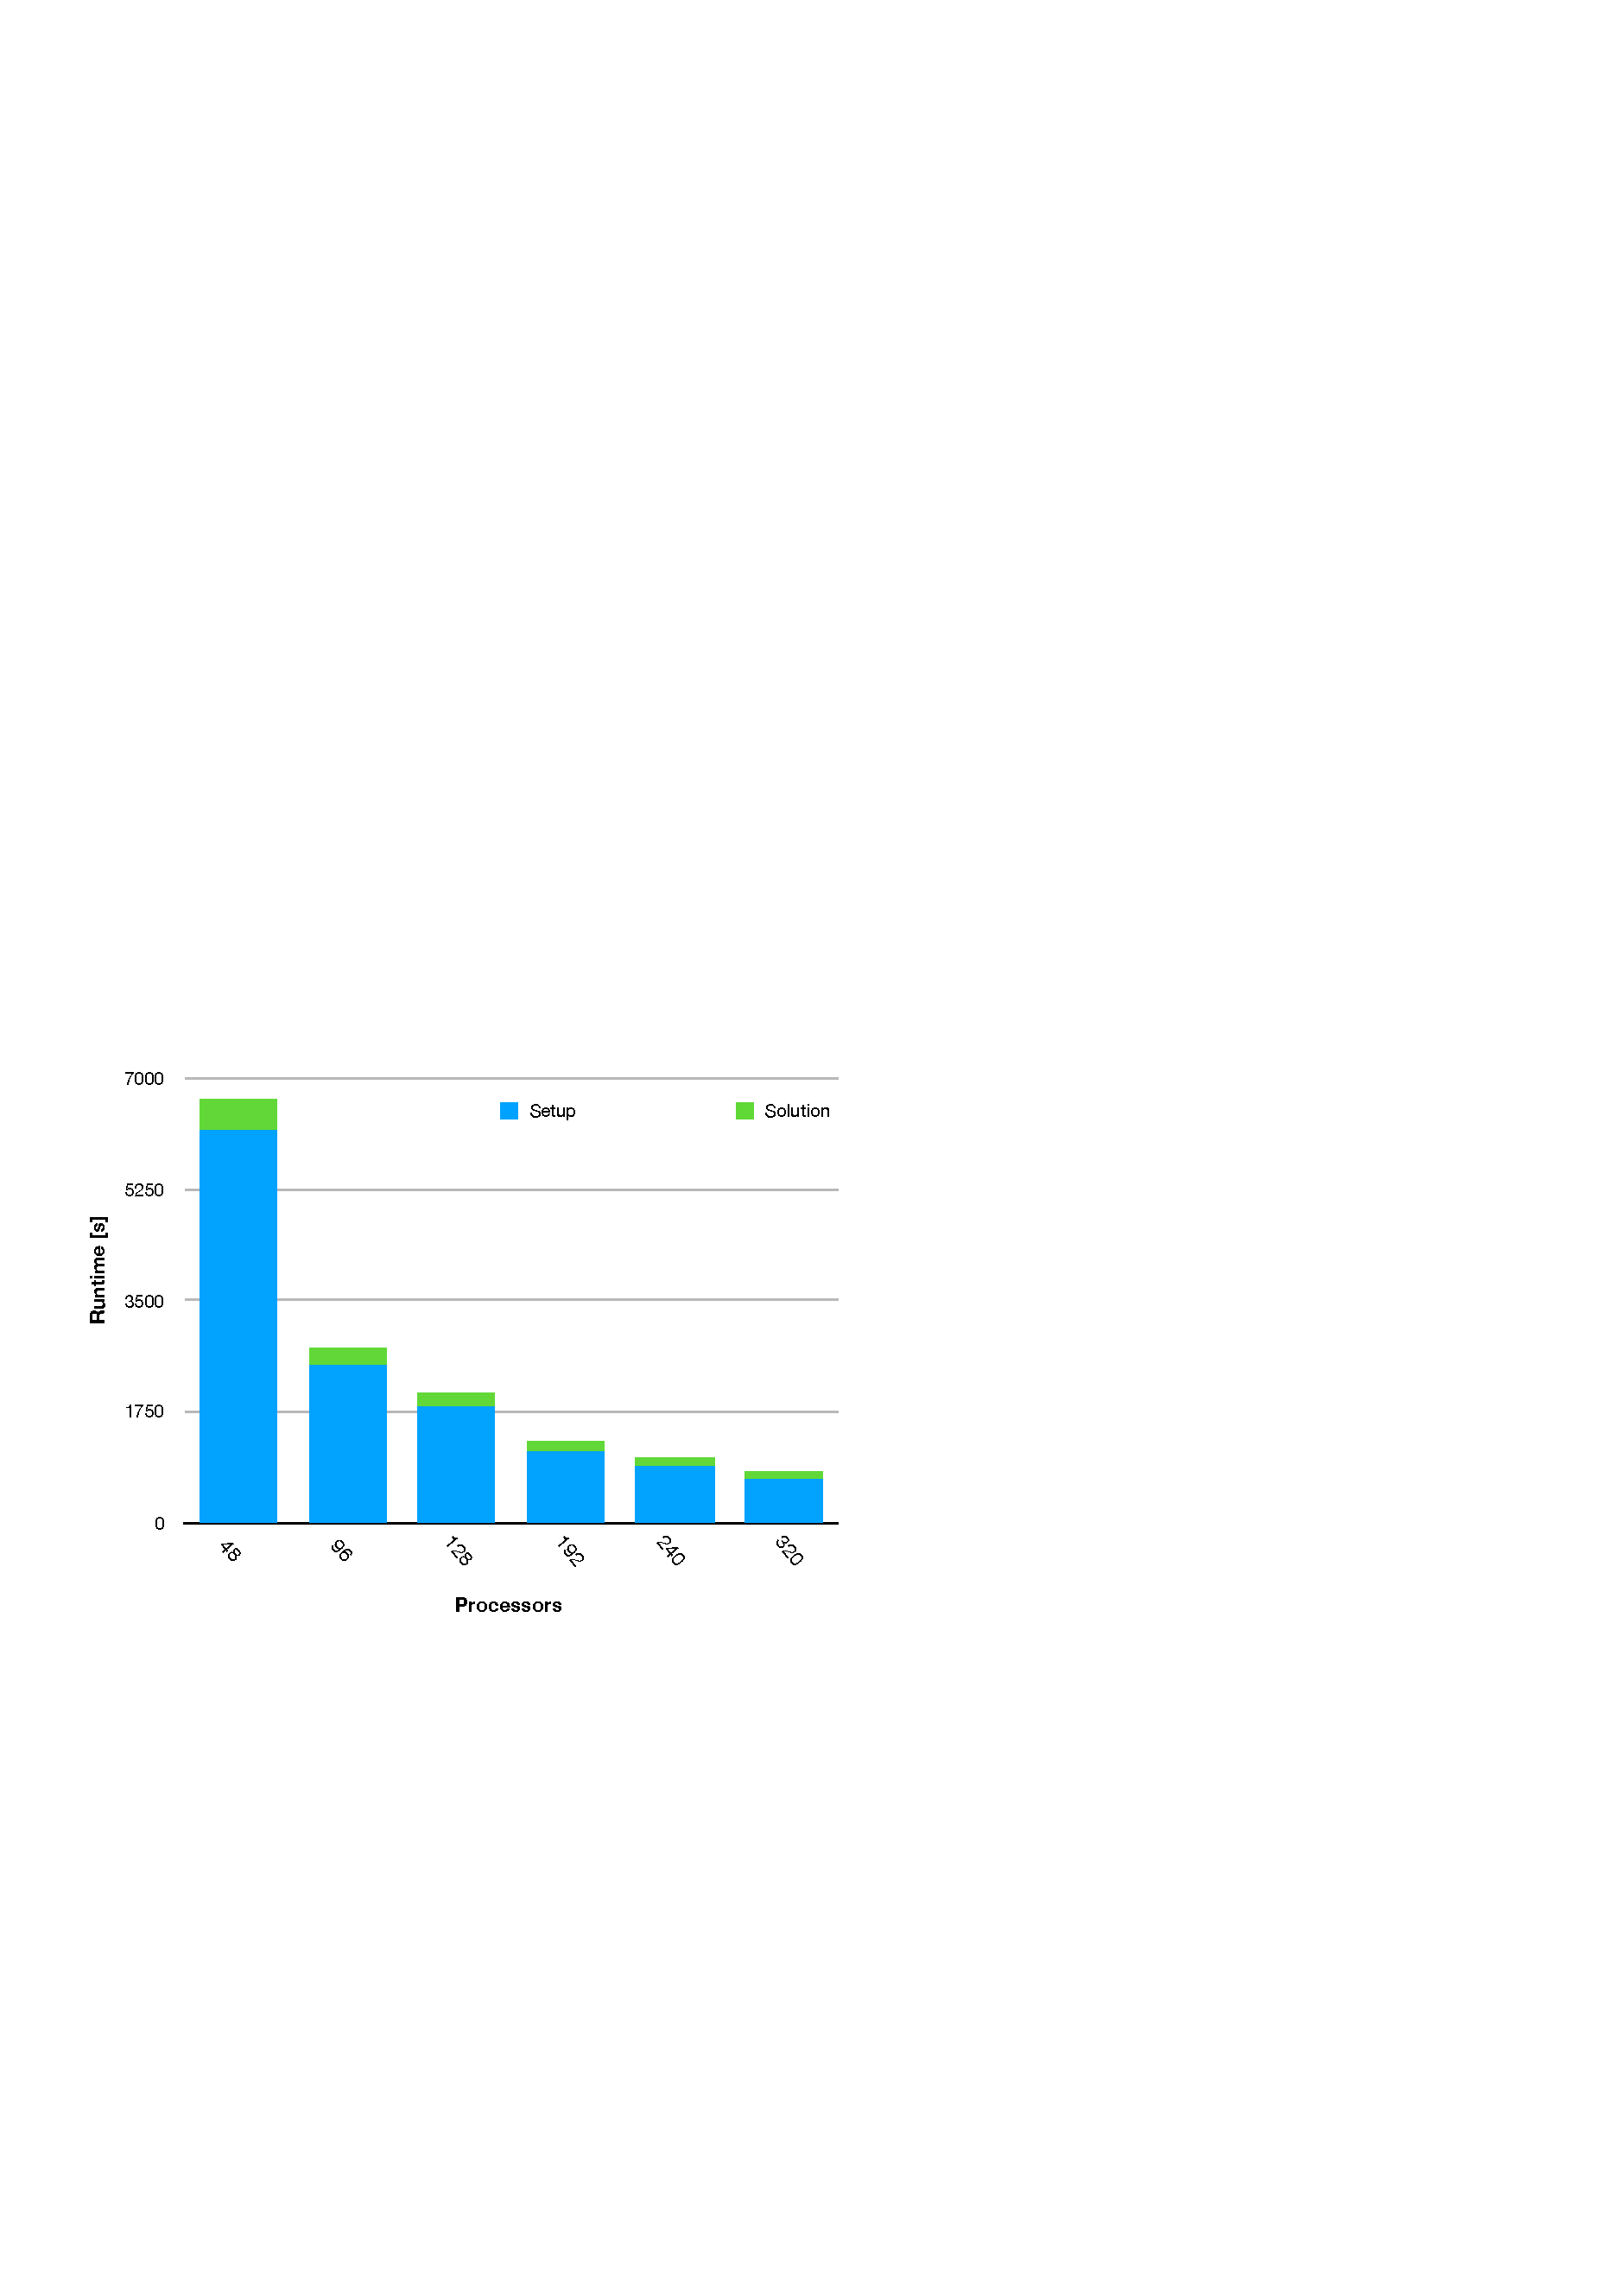
\includegraphics[width=.5\textwidth]{\figpath/Fig_cap_2/scal_ffddm_P2}}
\end{center}
\end{minipage}
\caption{Strong scalability of the ORAS preconditioner: $7.2$ millions of d.o.f and subdomains ranging from $48$ to $400$.}
\label{fig-scalability} 
\end{figure}

\begin{table}
	\begin{center}
		\begin{tabular}{cccc}
			 $\mathcal{N}$ & Factorization (s)  & GMRES (s)  & Total Step (s) \\ \hline \hline
			 48 & 6186.33  & 473.66  &  6659.99 \\
			 96 & 2468.68  & 283.099 &  2751.779 \\
			 128 & 1814.26 &  237.853 &   2052.113\\
			 192 & 1111.5  &   169.174 &  1280.674 \\
			 240 & 889.422  & 146.539 &  1035.961\\
			 320 & 674.204   &  114.346 & 788.55 \\
			 400 & 614.418  &  107.422 &  721.84\\ \hline
		\end{tabular}
	\end{center}
	\caption {Strong scaling experiment in 3D differentially heated cavity. $7.2$ millions of d.o.f and subdomains ranging from $48$ to $400$. }
	\label{tab-scalability}
\end{table}
